% This is the Amherst College LaTeX thesis template.
% See http://web.reed.edu/cis/help/latex.html for help. There are a
% great bunch of help pages there, with notes on
% getting started, bibtex, etc. Go there and read it if you're not
% already familiar with LaTeX.
%
% Any line that starts with a percent symbol is a comment.
% They won't show up in the document, and are useful for notes
% to yourself and explaining commands.
% Commenting also removes a line from the document;
% very handy for troubleshooting problems. -BTS

% As far as I know, this follows the requirements laid out in
% the 2002-2003 Senior Handbook. Ask a librarian to check the
% document before binding. -SN

%%
%% Preamble
%%
% \documentclass{<something>} must begin each LaTeX document
\documentclass[12pt,twoside]{amherstthesis}
% Packages are extensions to the basic LaTeX functions. Whatever you
% want to typeset, there is probably a package out there for it.
% Chemistry (chemtex), screenplays, you name it.
% Check out CTAN to see: http://www.ctan.org/
%%
\usepackage{graphicx,latexsym}
\usepackage{amsmath}
\usepackage{amssymb,amsthm}
\usepackage{longtable,booktabs,setspace}
\usepackage{chemarr} %% Useful for one reaction arrow, useless if you're not a chem major
\usepackage{rotating}

% Modified by CII
\usepackage[hyphens]{url}
\usepackage{hyperref}
\usepackage{lmodern}

% Added by CII (Thanks, Hadley!)
% Use ref for internal links
\renewcommand{\hyperref}[2][???]{\autoref{#1}}
\def\chapterautorefname{Chapter}
\def\sectionautorefname{Section}
\def\subsectionautorefname{Subsection}

\usepackage{caption}
\captionsetup{width=5in}

% \usepackage{times} % other fonts are available like times, bookman, charter, palatino

\title{A Simulation Study Using Random Graph Models to Fit Social Networks}
\author{Levi Lee}
% The month and year that you submit your FINAL draft TO THE LIBRARY (May or December)
\date{April 05, 2017}
\division{Statistics}
\advisor{Amy Wagaman}
%If you have two advisors for some reason, you can use the following
%\altadvisor{Your Other Advisor}
%%% Remember to use the correct department!
\department{Mathematics and Statistics}
% if you're writing a thesis in an interdisciplinary major,
% uncomment the line below and change the text as appropriate.
% check the Senior Handbook if unsure.
%\thedivisionof{The Established Interdisciplinary Committee for}
% if you want the approval page to say "Approved for the Committee",
% uncomment the next line
%\approvedforthe{Committee}

% Below added by CII

%%% Copied from knitr
%% maxwidth is the original width if it's less than linewidth
%% otherwise use linewidth (to make sure the graphics do not exceed the margin)
\makeatletter
\def\maxwidth{ %
  \ifdim\Gin@nat@width>\linewidth
    \linewidth
  \else
    \Gin@nat@width
  \fi
}
\makeatother

\renewcommand{\contentsname}{Table of Contents}

\setlength{\parskip}{0pt}

\providecommand{\tightlist}{%
  \setlength{\itemsep}{0pt}\setlength{\parskip}{0pt}}

\Acknowledgements{
This thesis would not have been possible without the support of so many
people. First and foremost, I would like to thank everyone currently
from the Mathematics and Statistics departments along with some previous
faculty as well. In particular, Professor Xiaofei (Susan) Wang and
Professor Eunice Kim were some of the first people that really got me
heavily involved with R and R-Studio through the coursework they
provided. I would never imagine that one day, I would be doing something
so advanced with such software. I would also like to thank my fellow
stats majors for always providing such amazing help when I get stuck. My
gratitude goes to Stephany Flores-Ramos '17, Melody Owen '17, Jordan
Browning '17, and Muling Si '17 for being such wonderful peers in
Advanced Data Analysis and for always bearing with me. Seeing how
wonderfully they all code really inspired me to improve my own skills as
well. Special thanks also goes to Ningyue (Christina) Wang '16 for all
the senior advice when I was a junior. To all the students, faculty, and
staff who knew I was working on this project, thank you for the constant
moral support. Those who also had a hand in helping with this project,
even if it was just moral support, are truly a cut above. I am
especially grateful to Roy Andrews '80 from the Writing Center, Caleb Ki
'17, and Azka Javaid '17 who were kind enough to read over my thesis and
provide valuable feedback. Special thanks to Nguyen (Johnson) Tran, a
childhood friend from back home in Florida, who was kind enough to gift
me a wonderful textbook on statistics, which proved to be very useful in
my research. I want to dedicate this next paragraph to my family.
Without their love and support, I would not be at Amherst today. Since
the day I started school, my parents have done everything in their power
to make sure the only thing I ever really need to focus on was my
education. Nothing could ever amount to the sacrifices they have made. I
now realize that being able to focus solely on academics was a privilege
that not everyone had. My penultimate thanks goes to Professor Nicholas
Horton, whom I have had the pleasure of having a professor for two
courses in a row. He is a professor, mentor, and coach who really has a
sense of the direction statistics is taking, and is really preparing us
all to ``think with data.'' Finally, I want to give my thanks to
Professor Amy Wagaman, who has been my ``three-times advisor'' for
Mathematics, Statistics, and my Mathematics Thesis. She has been an
amazing advior in all regards, and I cannot thank her enough for her
patience, understanding, and dedication to my learning. Working on such
a project has really been challenging, but was definitely the highlight
of my final year in college. It is thanks to her that I was able to
explore the facinating world of networks and pursue graduate study in
this field. I hope that this project has made her proud.
}

\Dedication{

}

\Preface{

}

\Abstract{
Networks see usage across many disciplines. This work focuses on social
networks, a category of networks which tend to exhibit some
characteristics unique to themselves. Is it possible to model social
networks despite their unique properties? To answer this question, we
begin with an overview of networks, including network statistics, and
graph models. We look at the Erdős-Rényi and Watts-Strogatz models as
well as exponential random graph models (ERGMs). We conduct a simulation
study where we apply various graph models to an observed network. Here,
we choose to analyze a component of the Facebook network. We compare the
network statistics of this Facebook network with those calculated from
graphs of parable magnitude simulated from their respective graph
models. We conclude that models such as the Erdős-Rényi and
Watts-Strogatz models do not accurately fit the Facebook network for
these network statistics. ERGMs that only use combinations of edge,
triangle, and k-star parameters also do not accurately model this
Facebook network as well. However, the results suggest that adding other
parameters can potentially improve simulation results.
}


%%
%% End Preamble
%%
%

\begin{document}

      \maketitle
  
  \frontmatter % this stuff will be roman-numbered
  \pagestyle{empty} % this removes page numbers from the frontmatter

      \begin{acknowledgements}
      This thesis would not have been possible without the support of so many
      people. First and foremost, I would like to thank everyone currently
      from the Mathematics and Statistics departments along with some previous
      faculty as well. In particular, Professor Xiaofei (Susan) Wang and
      Professor Eunice Kim were some of the first people that really got me
      heavily involved with R and R-Studio through the coursework they
      provided. I would never imagine that one day, I would be doing something
      so advanced with such software. I would also like to thank my fellow
      stats majors for always providing such amazing help when I get stuck. My
      gratitude goes to Stephany Flores-Ramos '17, Melody Owen '17, Jordan
      Browning '17, and Muling Si '17 for being such wonderful peers in
      Advanced Data Analysis and for always bearing with me. Seeing how
      wonderfully they all code really inspired me to improve my own skills as
      well. Special thanks also goes to Ningyue (Christina) Wang '16 for all
      the senior advice when I was a junior. To all the students, faculty, and
      staff who knew I was working on this project, thank you for the constant
      moral support. Those who also had a hand in helping with this project,
      even if it was just moral support, are truly a cut above. I am
      especially grateful to Roy Andrews '80 from the Writing Center, Caleb Ki
      '17, and Azka Javaid '17 who were kind enough to read over my thesis and
      provide valuable feedback. Special thanks to Nguyen (Johnson) Tran, a
      childhood friend from back home in Florida, who was kind enough to gift
      me a wonderful textbook on statistics, which proved to be very useful in
      my research. I want to dedicate this next paragraph to my family.
      Without their love and support, I would not be at Amherst today. Since
      the day I started school, my parents have done everything in their power
      to make sure the only thing I ever really need to focus on was my
      education. Nothing could ever amount to the sacrifices they have made. I
      now realize that being able to focus solely on academics was a privilege
      that not everyone had. My penultimate thanks goes to Professor Nicholas
      Horton, whom I have had the pleasure of having a professor for two
      courses in a row. He is a professor, mentor, and coach who really has a
      sense of the direction statistics is taking, and is really preparing us
      all to ``think with data.'' Finally, I want to give my thanks to
      Professor Amy Wagaman, who has been my ``three-times advisor'' for
      Mathematics, Statistics, and my Mathematics Thesis. She has been an
      amazing advior in all regards, and I cannot thank her enough for her
      patience, understanding, and dedication to my learning. Working on such
      a project has really been challenging, but was definitely the highlight
      of my final year in college. It is thanks to her that I was able to
      explore the facinating world of networks and pursue graduate study in
      this field. I hope that this project has made her proud.
    \end{acknowledgements}
  
  
  % Add table of abbreviations?

      \hypersetup{linkcolor=black}
    \setcounter{tocdepth}{2}
    \tableofcontents
  
      \listoftables
  
      \listoffigures
  
      \begin{abstract}
      Networks see usage across many disciplines. This work focuses on social
      networks, a category of networks which tend to exhibit some
      characteristics unique to themselves. Is it possible to model social
      networks despite their unique properties? To answer this question, we
      begin with an overview of networks, including network statistics, and
      graph models. We look at the Erdős-Rényi and Watts-Strogatz models as
      well as exponential random graph models (ERGMs). We conduct a simulation
      study where we apply various graph models to an observed network. Here,
      we choose to analyze a component of the Facebook network. We compare the
      network statistics of this Facebook network with those calculated from
      graphs of parable magnitude simulated from their respective graph
      models. We conclude that models such as the Erdős-Rényi and
      Watts-Strogatz models do not accurately fit the Facebook network for
      these network statistics. ERGMs that only use combinations of edge,
      triangle, and k-star parameters also do not accurately model this
      Facebook network as well. However, the results suggest that adding other
      parameters can potentially improve simulation results.
    \end{abstract}
  
  
  \mainmatter % here the regular arabic numbering starts
  \pagestyle{fancyplain} % turns page numbering back on

  \onehalfspacing
  
  \chapter*{Introduction}\label{introduction}
  \addcontentsline{toc}{chapter}{Introduction}
  
  Generally speaking, a \emph{network} is a collection of inter-related
  objects. This broad definition allows networks to be used in a variety
  of disciplines. We focus on \emph{social networks}, in which these
  objects are either individuals or groups (though these objects need not
  be human), called \emph{actors} and the relationships among them are
  called \emph{ties}. For people, these ties can be friendships,
  collaborations, and email exchanges, among other things. Social networks
  have been a growing field of study since the 1930s. Even before the
  computer age, people have observed unique relationships among
  individuals (Kolaczyk 2009 and Newman 2010). One famous example is
  Milgram's letter experiments. Travers \& Milgram (1967) considered 296
  individuals in Nebraska and Massachusetts who were instructed to
  construct chains of correspondence via letter until the correspondence
  reached a target person in Boston. Out of the 64 letter chains that
  succeeded, they discovered that, overall, these chains did not require
  that many people. Surprisingly, the median number of people the letters
  had to go through was approximately six, giving rise to the popular term
  ``six degrees of separation.''
  
  This phenomenon is not true for all types of networks; in fact, many
  social networks exhibit characteristics not seen in other types of
  networks. If we were given a social network, would it be possible then,
  for us to model social networks in spite of their unique properties?
  Models for networks certainly exist, but how accurate are they? It turns
  out that through a simulation study, we hope to find an answer or at
  least be pointed in the right direction. However, before heading
  straight to a simulation study, we must be careful in our approach.
  Exactly how do we mathematically define a network? What does a model for
  a network consist of? How would we measure accuracy for such models? We
  begin with some mathematical background before describing the components
  of the simulation study and we will see examples of social networks in
  subsequent sections.
  
  \section[Basic Terminology and Definitions]{\texorpdfstring{Basic
  Terminology and Definitions\footnote{The terms and definitions listed
    here are certainly not an exhaustive list. This section follows
    largely from Kolaczyk's \emph{Statistical Analysis of Network Data}.
    See Kolaczyk (2009) for more details.}}{Basic Terminology and Definitions}}\label{basic-terminology-and-definitions-1}
  
  In order to precisely define what we mean by a network, we borrow much
  of the mathematical terminology for networks and network statistics from
  graph theory. More formally, a network is a collection of vertices and
  edges. It is a \emph{graph}, that is, a structure denoted \(G = (V, E)\)
  such that \(E\) is the set of edges and \(V\) is the set of vertices.
  The \emph{order} of a graph \(G\) is defined to be the number of
  vertices in \(G\), denoted \(N_V = |V|\). Similarly, the \emph{size} of
  \(G\) is the number of edges in \(G\), denoted \(N_E = |E|\).
  
  Each edge connects two vertices, and so for any two vertices
  \(i, j \in V\), if \(i\) and \(j\) have a connection then the ordered
  pair \(\{i, j\} = e \in E\). In this case, we say \(i\) is
  \emph{adjacent} to \(j\) and that \(i\) and \(j\) are \emph{neighbors}.
  That is, \(\{i, j\}\) is the same as \(\{j, i\}\). Such a graph is
  called \emph{undirected} (or \emph{non-directed}). Graphs that have
  ordering to their edges, that is, where \(\{i, j\} \in E\) is different
  from \(\{j, i\} \in E\), are called \emph{directed graphs} (or
  \emph{digraphs}), and the edges in a directed graph are called
  \emph{directed edges} (or \emph{arcs}). For example, friendships on
  Facebook are undirected. This is because friendships on this platform
  are mutual--if person A is friends with person B, it also means that
  person B is friends with person A. Followers on Twitter, on the other
  hand, are directed. If person A is following person B, it does not
  necessarily mean that person B is following person A (Baumer, Kaplan, \&
  Horton 2017). Our focus will be on graphs whose edges are undirected.
  
  We can also represent a network with just the connections that are
  present (or not present) between vertices by using an \emph{adjacency
  matrix}. Given a graph \(G = (V, E)\), the adjacency matrix
  \(\textbf{A}\) is an \(N_V\) x \(N_V\) matrix where
  
  \[ A_{ij} = \begin{cases}
      1 & \text{if } \{i, j\} \in E \\
      0 & \text{otherwise.} 
    \end{cases}
  \]
  
  Matrix \(\textbf{A}\) is symmetric if \(G\) is a undirected graph, but
  this may not necessarily be the case if \(G\) is a directed graph. This
  is because \(\{i, j\} \in E\) does not necessarily guarantee that
  \(\{j, i\} \in E\) for directed graphs.
  
  While the adjacency matrix \(\textbf{A}\) is a data structure that fully
  characterizes a graph, for large \(N_{V}\), size and reading time on the
  part of the computer can become an issue very quickly, especially in the
  context of working with data structures and particular algorithms. For a
  graph with \(N_{V}\) vertices, the corresponding adjacency matrix will
  have \(N_{V}^{2}\) elements. Thus, we can also consider an alternative:
  an \emph{edge list} is a two-column list of all the edges and their
  corresponding vertices present in a graph. More often than not, a graph
  will not have an edge between every pair of vertices, so it is more
  often the case that using an edge list will mean we are dealing with
  strictly less than \(N_{V}^{2}\) elements. Larger networks, as we will
  soon see, are more often than not represented with an edge list.
  
  To describe how to move about in a network, we define a \emph{walk} in
  graph \(G\) to be a sequence that begins and ends with two vertices and
  alternates between vertices and edges. The sequence
  \((a_0, e_1, a_1, e_2, ..., v_{l-1}, e_l, v_l)\) denotes one path from
  vertex \(a_0\) to vertex \(a_l\), where for all \(e_i \in E\), \(e_i\)
  connects points \(a_{i-1}\) and \(a_i \in V\). Using this notation, we
  define the \emph{length} of the walk to be the value \(l\). More refined
  than a walk, a \emph{trail} is defined to be a walk in which the
  sequence does not traverse through the same edge more than once. And
  even more refined still is a \emph{path} in which a walk does not travel
  through the same vertex twice.
  
  A vertex \(j\) is \emph{reachable} from another vertex \(i\) if there is
  a walk from \(i\) to \(j\). \(G\) is \emph{connected} if all vertices in
  \(G\) are reachable by some other vertex in \(G\). A \emph{component} is
  a subgraph that is maximally connected. The length of the shortest
  path(s) between any two vertices is defined to be the \emph{distance}
  (or \emph{geodesic distance}) between vertices. This distance is
  infinite if no path between two particular vertices exist, that is, they
  are located on different components. The \emph{diameter} is the longest
  (geodesic) distance achieved in a graph. In a digraph, a \emph{directed
  walk} is analogous to a walk, but uses arcs to get from one vertex to
  another.
  
  A graph is \emph{complete} if every vertex has an edge with all other
  vertices in the graph. An undirected graph is \emph{simple} if it has no
  \emph{loops} and \emph{multi-edges}, meaning vertices do not have an
  edge that points to itself and any pair of vertices do not have more
  than one edge between them. Edges on a simple graph are called
  \emph{proper edges}. A \emph{clique} is a graph or subgraph that is
  complete. A graph is \emph{regular} if each vertex has the same
  \emph{degree}. That is, each vertex has the same number of edges
  connecting to it. Degree is usually denoted \(k\), and a particular
  vertex with a degree \(k\) is called a \emph{\(k\)-star}.
  
  Connectedness and simpleness are very important characteristics of
  networks as many of the descriptive statistics that we will see can only
  be applied graphs with such properties. In fact, our focus will also be
  limited to simple and connected graphs.
  
  A graph can contain other information or data, called \emph{attributes},
  beyond just the collection of vertices and edges. Incorporating these
  attributes, otherwise known as \emph{decorating} a graph, can occur in
  both the vertices, edges, and even in the entire graph itself. For
  example, it is possible to assign \emph{edge weights} to each edge. That
  is, we assign an edge weight \(w_e\) to \(e = \{i, j\} \in E\). A
  \emph{weighted graph} is a graph whose edges include weights that are
  nonzero and between \(0\) and \(1\). Edge and vertex attributes can be
  \emph{discrete} or \emph{continuous}. An example of a discrete attribute
  is a binary case of positive or negative relationship between pairs of
  vertices. An example of a continuous attribute would be the strength (or
  weight) of the relationship between pairs.
  
  \section{Example 1: Zachary's Karate
  Club}\label{example-1-zacharys-karate-club}
  
  One famous (or infamous) social network, called ``the karate club of
  Zachary,'' was observed by anthropologist Zachary (1977). The vertices
  in this network indicate the 34 individual actors (that is, members) of
  the karate club while the edges indicate the 78 social ties among pairs
  of the members. Figure 1 provides a visual summary of the karate network
  data. As shown by the colors of the vertices, the club, at this
  particular moment in time, is being divided into two factions centering
  around two vertices as labeled by letters--the master and primary
  disciple of the dojo.
  
  \begin{figure}[htbp]
  \centering
  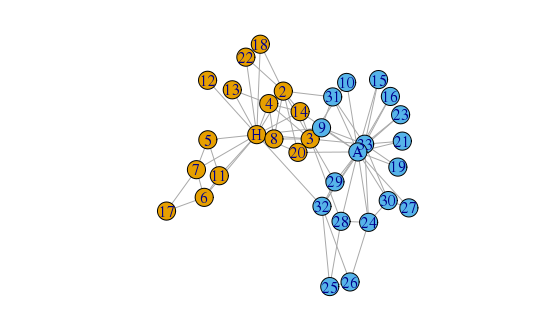
\includegraphics{figure/01karateplot.png}
  \caption{Zachary's Karate Club (\(N_V = 34\), \(N_E = 78\))}
  \end{figure}
  
  It is possible to display more than just the actors and their
  relationships. We can provide more information by assigning other visual
  cues--such as vertex shapes to determine gender, vertex size to indicate
  belt rank, and edge weights to determine the strength of the social
  tie--to each member.
  
  \section{Example 2: Lazega's Law Firm}\label{example-2-lazegas-law-firm}
  
  Consider a network of actors that reflects the relational data collected
  by Lazega \& Pattison (1999) of a New England law firm of 36 lawyers
  (actors) and 115 work collaborations (ties). In Figure 2, each lawyer is
  individually labeled with smaller numbers indicating seniority. Shapes
  for each lawyer indicate the type of practice: litigation (circles) and
  corporate (squares). The shapes' sizes indicate the relative number of
  years of having been with the law firm. Color is used to indicate office
  location (red, blue, and yellow). The graph below provides a visual
  summary of the lawyer network data.
  
  \begin{figure}[htbp]
  \centering
  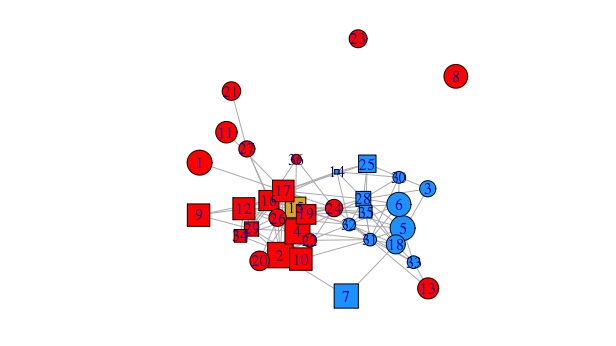
\includegraphics{figure/02lawyerplot.png}
  \caption{Lazega's Law Firm (\(N_V = 36\), \(N_E = 115\))}
  \end{figure}
  
  We can also continue adding layers of data to this visual as well. For
  example, if the appropriate data was recorded, it is possible quantify
  and/or qualify the collaborations between the lawyers. We can apply
  weights to give an idea of how frequently any pair of lawyers interacted
  with each other in this resource exchange; we can even apply line types
  (solid, dashed, double-dashed, etc.) to indicate how this collaboration
  took place: was it done in person, through the phone, through email, or
  some combination of the three?
  
  \section{Modeling Real-World
  Networks}\label{modeling-real-world-networks}
  
  As noted earlier, one topic of study with practical applications is
  using models to ``model'' observed networks. These are more formally
  known as \emph{graph models} and for now, we can think of them as ways
  to emulate graphs. Which models can generate graphs that are visually
  and structurally similar to the social networks that we observed? In
  reality, there are many graph models to choose from. With a network
  chosen, one approach is through a simulation study in which we can
  generate graphs from different graph models and compare
  \emph{descriptive network statistics} between the simulated graphs and
  the observed graphs to see how accurate these graph models are.
  
  Being able to model observed networks would benefit many fields. By
  accurately predicting how networks form, it may be possible to
  understand how friendships among people form or even how information is
  spread across people. More generally, we can improve traffic flow,
  provide better product suggestions to online shoppers, and help prevent
  the spread of diseases.
  
  In this thesis, we provide a general overview about network statistics
  and graph models, followed by a simulation study that tests different
  graph models and see how well they ``fit'' a target social network of
  our choosing. In Chapter 1, we focus on various network statistics.
  These statistics have direct (but sometimes non-trivial) analogs to the
  measures of spread and central tendency seen in introductory Statistics.
  For example, we will see that \emph{centrality}, a measure of importance
  of vertices in graphs, is similar to the arithmetic mean for a set. In
  Chapter 2, we focus on describing various graph models, such as the
  Erdős-Rényi and Watts-Strogatz models and several different exponential
  random graph models (ERGMs). These graph models will be used to fit a
  social network of our choosing. We will be using an undirected, simple,
  and connected component of the Facebook network, which consists of
  \(4039\) vertices and \(88234\) edges. Chapter 3 describes our
  simulation study and results. We compare the network statistics of our
  simulated graphs to those of the observed network. We conclude with
  Chapter 4, which describes some of the limitations in this study and
  potential future work.
  
  \chapter{Descriptive Network
  Statistics}\label{descriptive-network-statistics}
  
  Descriptive statistics for networks are somewhat analogous to those seen
  in elementary statistics. In fact, we have seen a few already in the
  section of basic terminology in our Introduction. We describe a few
  below and explain them in the context of Zachary's karate club and
  Lazega's lawyer firm.\footnote{Just like the basic terminology for
    networks, the list of network statistics seen here is not exhaustive.
    For more details, please refer to Kolaczyk (2009), Newman (2010) and
    Csárdi \& Nepusz (2006).} We will use these network statistics to
  characterize our component of the Facebook network as well as the
  networks generated by the graph models described in the next chapter. As
  a result, we then have a way to compare different networks, which is
  similar to how elementary descriptive statistics allow us to compare
  across different data sets.
  
  \begin{longtable}[]{@{}lrr@{}}
  \caption{Some average network statistics for the karate and lawyer
  networks \label{tab:avgnetstats}}\tabularnewline
  \toprule
  \begin{minipage}[b]{0.29\columnwidth}\raggedright\strut
  Network Statistic\strut
  \end{minipage} & \begin{minipage}[b]{0.29\columnwidth}\raggedleft\strut
  Zachary's Karate Club\strut
  \end{minipage} & \begin{minipage}[b]{0.23\columnwidth}\raggedleft\strut
  Lazega's Law Firm\strut
  \end{minipage}\tabularnewline
  \midrule
  \endfirsthead
  \toprule
  \begin{minipage}[b]{0.29\columnwidth}\raggedright\strut
  Network Statistic\strut
  \end{minipage} & \begin{minipage}[b]{0.29\columnwidth}\raggedleft\strut
  Zachary's Karate Club\strut
  \end{minipage} & \begin{minipage}[b]{0.23\columnwidth}\raggedleft\strut
  Lazega's Law Firm\strut
  \end{minipage}\tabularnewline
  \midrule
  \endhead
  \begin{minipage}[t]{0.29\columnwidth}\raggedright\strut
  Transitivity (Global)\strut
  \end{minipage} & \begin{minipage}[t]{0.29\columnwidth}\raggedleft\strut
  0.256\strut
  \end{minipage} & \begin{minipage}[t]{0.23\columnwidth}\raggedleft\strut
  0.389\strut
  \end{minipage}\tabularnewline
  \begin{minipage}[t]{0.29\columnwidth}\raggedright\strut
  Transitivity (Local)\strut
  \end{minipage} & \begin{minipage}[t]{0.29\columnwidth}\raggedleft\strut
  0.588\strut
  \end{minipage} & \begin{minipage}[t]{0.23\columnwidth}\raggedleft\strut
  0.487\strut
  \end{minipage}\tabularnewline
  \begin{minipage}[t]{0.29\columnwidth}\raggedright\strut
  Avg. Path Length\strut
  \end{minipage} & \begin{minipage}[t]{0.29\columnwidth}\raggedleft\strut
  2.408\strut
  \end{minipage} & \begin{minipage}[t]{0.23\columnwidth}\raggedleft\strut
  2.144\strut
  \end{minipage}\tabularnewline
  \begin{minipage}[t]{0.29\columnwidth}\raggedright\strut
  Diameter\strut
  \end{minipage} & \begin{minipage}[t]{0.29\columnwidth}\raggedleft\strut
  13\strut
  \end{minipage} & \begin{minipage}[t]{0.23\columnwidth}\raggedleft\strut
  5\strut
  \end{minipage}\tabularnewline
  \bottomrule
  \end{longtable}
  
  \section{Transitivity}\label{transitivity}
  
  \emph{Transitivity}, otherwise known as the \emph{clustering
  coefficient}, is the probability that adjacent vertices of a particular
  vertex are connected. In other words, this value provides a sense of how
  well-connected the graph is. A higher transitivity implies a graph
  having many vertices in proximity with each other with edges connecting
  all of them. Different kinds of transitivity exist and the choice of
  which one to observe depends largely on whether one wishes to talk about
  the network globally or locally (Kolaczyk 2009). Both are explained
  below, but for the sake of choosing one for our analyses, we will focus
  on the \emph{local average transitivity}.
  
  Globally speaking, this value is the ratio of connected triples to all
  possible triangles in the graph. We define a \emph{triangle} (or
  \emph{triad}) as subgraphs with three vertices; if these vertices are
  connected by two edges, it is a \emph{connected triple}. Formulaically,
  the clustering coefficient, denoted with uppercase \(C\), is
  
  \[C = \frac {(\text{number of triangles}) \times 3} {\text{number of connected triples}}.\]
  
  The factor of \(3\) represents the fact that a triangle is counted three
  times when we consider the number of triples in the network.
  
  The local transitivity is calculated for each vertex in the graph and is
  the ratio of triangles connected to a particular vertex to the connected
  triples centered on the vertex. For a particular vertex \(i\), the local
  transitivity is denoted as
  
  \[ C_{i} = \frac {(\text{number of pairs of neighbors of } i \text{ that are connected})} {(\text{number of pairs of neighbors of } i)}.\]
  The local average transitivity then, is the average of the local
  transitivity values for each vertex in the graph.
  
  In the Zachary's karate club and Lazega's law firm examples, the local
  average transitivity values are: 0.588 and 0.487, respectively, and the
  global transitivity values are 0.256 and 0.389, respectively. This means
  that while the lawyer network has a greater amount of clustering than
  the karate network overall, locally speaking, there are more vertices in
  the karate network that form many triangles and connected triples
  compared to the lawyer network. However, social networks in general tend
  to have higher-than-average transitivity values compared to networks of
  other types.
  
  \section{Average Path Length}\label{average-path-length}
  
  \emph{Average path length} (or \emph{average geodesic distance}) is the
  average of the shortest paths of all distinct pairs of vertices in the
  network. This is also a commonly used statistic for social networks
  since average path lengths tend to be much less than what we would
  expect in these networks than if the edges were placed between vertices
  randomly (Kolaczyk 2009).
  
  The karate network has an average path length of 2.408 while the lawyer
  network has an average path length of 2.144. This means that in both
  cases, any two people in both networks are separated by an average of a
  little over two people. With Milgram's experiment and the concept of six
  degrees of separation in mind, we can tell that these are reasonable
  values indicative of social networks, which are known to have small
  average path lengths regardless of the number of individuals in the
  network (Newman 2010).
  
  \section{Diameter}\label{diameter}
  
  The \emph{diameter} of a graph is the longest of all the shortest paths
  between distinct pairs of vertices. This value gives our graph a notion
  of distance. Unlike average path length, however, diameter can be
  unpredictable at times since this value can be an outlier compared to
  other path lengths in the network (Kolaczyk 2009).
  
  The diameters of the karate and lawyer networks are 13 and 5,
  respectively. In the law firm of 36 people, people are, maximally, only
  as far as five people away from each other, but for the karate network,
  even in a group of 34, there exist two club members that do not have a
  direct relationship with each other and are separated by 12 other
  members (that is, 13 ties in between).
  
  \section{Centrality}\label{centrality}
  
  \emph{Centrality} assigns a measure of ``importance'' to each vertex in
  the network. It is similar to the measures of central tendency seen in
  elementary statistics. People have proposed different types of
  centrality, some of which are discussed below. We assume our graph \(G\)
  is undirected (Kolaczyk 2009).
  
  \emph{Vertex degree} (or \emph{degree centrality}) is perhaps the most
  common type of centrality. It is not surprising that vertices with
  higher vertex degrees are considered to be more central to the network
  than those with lower vertex degrees. In fact, one common characteristic
  among real-world networks is that their degree distributions tend to
  have an unusually high number of such vertices. The mean of the vertex
  degrees of all the vertices of the graph yields the \emph{mean} (or
  \emph{average}) \emph{degree}, often denoted with lowercase \(c\).
  
  \emph{Closeness centrality} measures how close a vertex is to other
  vertices based on the inverse of the total distance of the vertex from
  all others. Closeness centrality is computed as:
  
  \[c_{Cl}(i) = \frac {1} {\sum_{j \in V}^{} d(i, j)},\]
  
  where \(dist(i,j)\) is the geodesic distance between the vertices
  \(i,j \in V\). To compare across graphs and with other centrality
  measures, this measure is often normalized to lie in the interval
  \([0,1]\) by multiplying by a factor of \(N_V - 1\).
  
  \emph{Betweenness centrality} measures are aimed at summarizing the
  extent to which a vertex is located between other pairs of vertices. The
  most commonly used version of betweenness centrality is
  
  \[c_{B}(i) = \sum_{g \neq h \neq i \in V}^{} \frac {\sigma(g,h|i)} {\sigma(g,h)},\]
  
  where \(\sigma(g,h|i)\) is the total number of shortest paths between
  \(g\) and \(h\) that pass through \(i\), and
  \(\sigma(g,h) = \sum_{i \in V}^{} \sigma(g,h|i)\). If the shortest paths
  are unique, \(c_{B}(i)\) just counts the number of shortest paths going
  through \(i\). This centrality can be normalized by dividing by a factor
  of \(\frac {(N_V - 1)(N_V - 2)} {2}\).
  
  \emph{Eigenvector centrality} is based on the idea of ``status,''
  ``prestige,'' or ``rank;'' the more central the neighbors of a vertex
  are, the more central that vertex itself is. One definition of such a
  centrality measure is
  
  \[c_{Ei}(i) = \alpha \sum_{\{i,j\} \in E}^{} c_{Ei} (u).\]
  
  The vector \(c_{Ei} = (c_{Ei}(1), ..., c_{Ei}(N_V))^T\) is the solution
  to the eigenvalue problem
  \(\textbf{A}\textbf{c}_{Ei} = \alpha^{-1}\textbf{c}_{Ei}\), where
  \(\textbf{A}\) is the adjacency matrix for network graph \(G\).
  
  Centrality measures, like the local average transitivity, provide a
  value for each vertex in the graph. Because of this, we can obtain an
  overall centrality measure for the graph as a whole if we average the
  values for each vertex.
  
  \begin{longtable}[]{@{}lll@{}}
  \caption{Average centrality measures for the karate and lawyer networks
  \label{tab:avgcent}}\tabularnewline
  \toprule
  \begin{minipage}[b]{0.27\columnwidth}\raggedright\strut
  Network Statistic\strut
  \end{minipage} & \begin{minipage}[b]{0.29\columnwidth}\raggedright\strut
  Zachary's Karate Club\strut
  \end{minipage} & \begin{minipage}[b]{0.23\columnwidth}\raggedright\strut
  Lazega's Law Firm\strut
  \end{minipage}\tabularnewline
  \midrule
  \endfirsthead
  \toprule
  \begin{minipage}[b]{0.27\columnwidth}\raggedright\strut
  Network Statistic\strut
  \end{minipage} & \begin{minipage}[b]{0.29\columnwidth}\raggedright\strut
  Zachary's Karate Club\strut
  \end{minipage} & \begin{minipage}[b]{0.23\columnwidth}\raggedright\strut
  Lazega's Law Firm\strut
  \end{minipage}\tabularnewline
  \midrule
  \endhead
  \begin{minipage}[t]{0.27\columnwidth}\raggedright\strut
  Degree\strut
  \end{minipage} & \begin{minipage}[t]{0.29\columnwidth}\raggedright\strut
  4.588\strut
  \end{minipage} & \begin{minipage}[t]{0.23\columnwidth}\raggedright\strut
  6.389\strut
  \end{minipage}\tabularnewline
  \begin{minipage}[t]{0.27\columnwidth}\raggedright\strut
  Closeness Cen.\strut
  \end{minipage} & \begin{minipage}[t]{0.29\columnwidth}\raggedright\strut
  0.005\strut
  \end{minipage} & \begin{minipage}[t]{0.23\columnwidth}\raggedright\strut
  0.007\strut
  \end{minipage}\tabularnewline
  \begin{minipage}[t]{0.27\columnwidth}\raggedright\strut
  Betweenness Cen.\strut
  \end{minipage} & \begin{minipage}[t]{0.29\columnwidth}\raggedright\strut
  26.194\strut
  \end{minipage} & \begin{minipage}[t]{0.23\columnwidth}\raggedright\strut
  17.833\strut
  \end{minipage}\tabularnewline
  \begin{minipage}[t]{0.27\columnwidth}\raggedright\strut
  Eigenvector Cen.\strut
  \end{minipage} & \begin{minipage}[t]{0.29\columnwidth}\raggedright\strut
  0.377\strut
  \end{minipage} & \begin{minipage}[t]{0.23\columnwidth}\raggedright\strut
  0.458\strut
  \end{minipage}\tabularnewline
  \bottomrule
  \end{longtable}
  
  \autoref{tab:avgcent} above shows the average centrality measures for
  both the karate and lawyer networks. Because each type of centrality is
  measuring the importance of vertices differently, it comes as no
  surprise that all of the average centrality values within one network
  will be different from each other. These average values, however, do not
  give any indication of which, or how many, vertices in the network are
  important. We also note that the centrality measures here are not
  scaled. However, because the scaling factors are dependent on the number
  of vertices in the network, it is possible for us to compare between
  these two networks, as both have approximately the same number of
  vertices.
  
  Additionally, the use of an average means that the value can be
  subjected to some very drastic outliers that could potentially skew its
  value. However, from \autoref{tab:avgcent}, we see that lawyers in the
  law firm tend to have higher degrees, closeness centrality, and
  eigenvector centrality on average than the karate club. This means that,
  on average the lawyers in this firm have a lot of ties in the firm, are
  very well connected, and have a relatively high rank amongst their peers
  when compared to those in the karate club. The high betweenness
  centrality in the karate club indicates that there are a few members (in
  particular, the dojo's master and the disciple) who tend to have
  connections with members that do not have connections with each other.
  These centrality measures make sense since those in the company are
  probably more likely to know one another than those in the karate club
  who may only be on close terms with the master.
  
  We will use these seven network statistics listed above in our
  simulation study. By calculating these values from our observed network,
  it is possible for us to compare our network with graphs simulated from
  our graph models.
  
  \chapter{Graph Models}\label{graph-models}
  
  A \emph{graph model} takes in fixed parameters that generate a graph
  that can vary in structure with each iteration. Equivalently, it is also
  possible to consider a model for a graph as a collection, or
  \emph{ensemble},
  
  \[\{\mathbb{P}_{\theta}(G), G \in \mathcal{G}: \theta \in \Theta\}\]
  
  in which \(G\) is a collection or ensemble of possible graphs,
  \(P_\theta\) is a \emph{probability distribution} on \(G\) (that is, a
  function that assigns a value for very possible graph that G can be,
  whose total sums to \(1\)), and \(\theta\) is a vector of parameters
  that describe the graphs that G can be, ranging over possible parameters
  in \(\Theta\) (Kolaczyk 2009, Newman 2010).\footnote{Many of the
    explanations and derivations for the Erdős-Rényi and Watts-Strogatz
    networks here follow from Newman (2010). Much of the explanation about
    exponential random graph models (ERGMs) follows largely from C. Butts
    et al. (2015), David R. Hunter, Handcock, Butts, Goodreau, \& Morris
    (2008a), and Jackson (2013).}
  
  \section{Erdős-Rényi Model}\label{erdos-renyi-model}
  
  The \emph{Erdős-Rényi model} (also known as the
  \emph{Erdős-Rényi-Gilbert model}) is one of the most studied graph
  models.\footnote{Many other names for this model exist, such as
    \emph{Bernoulli model} (or \emph{Bernoulli random graph}) and the
    \emph{Poisson random graph} due to the properties of its degree
    distribution, as we will see. In fact, Paul Erdős and Alfréd Rényi
    were not the first to study or discover this model. According to
    Newman (2010), the earliest known study of this model is by Ray
    Solomonoff and Anatol Rapoport in 1951.} It is also one of the
  simplest, as it takes only two parameters. The model \(G(N_V, N_E)\),
  first suggested by Gilbert (1959), takes in \(N_V\), the number of
  nodes, and \(N_E\) the number of edges. Erdős and Rényi (1959, 1960,
  1964) considered the model of the form \(G(N_{V}, p)\), where instead of
  using the number of edges, the probability of an edge forming between
  any pairs of nodes is fixed. Our focus is on the latter model. It is
  clear that, on average, the \(G(N_{V}, p)\) model would comprise of many
  more networks than the \(G(N_V, N_E)\) model, as the number edges is not
  fixed. This allows us to consider a larger number of networks with
  similar network statistics seen in Chapter 1. However, while unlikely,
  it is possible to obtain a graph with no edges or all possible edges
  from the \(G(N_{V}, p)\) model (Newman 2010).
  
  \begin{figure}[htbp]
  \centering
  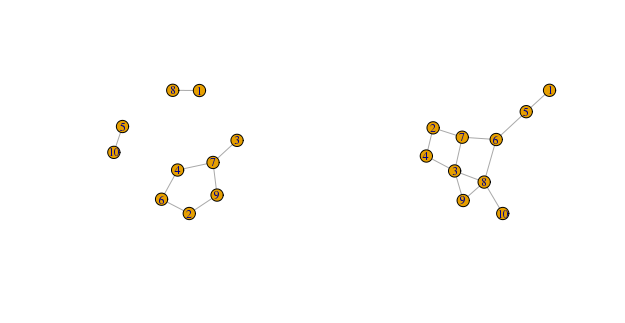
\includegraphics{figure/21erdosrenyiexample.png}
  \caption{Examples of graphs generated from the Erdős-Rényi model. Left
  and Right: \(N_V = 10\), \(p = 0.25\).}
  \end{figure}
  
  In the \(G(N_{V}, p)\) model, graphs constructed according to this model
  could potentially look every different from each other. This goes back
  to the idea that a graph model can be thought of as a probability
  distribution over an ensemble of networks, and all networks in this
  particular ensemble have equal probability of being chosen. We
  immediately see a potential drawback in graphs generated from this
  model: it places no significance on structures that we may see in our
  observed social networks--such as having high clustering, cliques, and
  connected components. However, because of the random placement of the
  edges across the vertices, values such as average path length are often
  quite small, even for large graphs (Newman 2010). This is one of many
  things that characterize social networks and is a primary the motivation
  for using this model for our analysis (even as a starting point).
  
  The Erdős-Rényi model has other nice properties, some of which we
  discuss below. Even with only two parameters \(N_{V}\) and \(p\) on
  hand, we can still create formulas that allow us to calculate various
  network statistics, such as average degree and clustering coefficient,
  and describe the model's degree distribution.
  
  As indicated earlier, the \(G(N_V, p)\) model is the collection of
  simple graphs with exactly \(N_{V}\) vertices, meaning that a particular
  simple graph \(g\) with exactly \(N_V\) vertices has probability
  \[P(G = g) = p^{N_E}(1 - p)^{\left({N_V \choose 2} - N_E \right)}\] of
  being picked. For precisely \(N_E\) edges, there are
  \({{N_{V} \choose 2} \choose N_{E}}\) ways to arrange the \(N_{E}\)
  edges among the \({N_V \choose 2}\) possible edges. Thus, the total
  probability of a random graph \(G\) with \(N_{E}\) edges and \(N_{V}\)
  vertices is
  \[P(G) = {{N_{V} \choose 2} \choose N_{E}}p^{N_E}(1 - p)^{{N_V \choose 2} - N_E}\]
  This, however, is simply a binomial distribution, where we have some
  probability of success (\(p\)), two possible outcomes (edge formation or
  no edge formation), a finite number of trials (\({N_{V} \choose 2}\)
  possible edges), and \({{N_{V} \choose 2} \choose N_{E}}\) different
  ways in which the outcomes can be arranged. Using this, the mean value
  of \(N_E\) for the model is then a weighted average. It is the sum of
  the products of every possible number of edges \(N_E\) and the total
  probability that a graph with \(N_{V}\) vertices and \(N_{E}\) edges
  appears, \(P(N_{E})\). However, because we know the probability of an
  edge forming, the mean number of edges would equal to the product of the
  total number of possible vertices \({N_{V} \choose 2}\) and the
  probability \(p\). This makes sense as we can expect that \(100p\)
  percent of the possible edges in the graph to actually have edges. Thus,
  the mean number of edges \(\langle N_{E} \rangle\) for a random graph
  \(G\) is
  \[ \langle N_{E} \rangle = \sum_{N_{E}=0}^{{N_{V} \choose 2}} N_{E}P(N_{E}) = {N_{V} \choose 2}p\]
  
  For a graph with exactly \(N_{E}\) edges, it is easy to see that the
  mean degree is \(\frac {2N_{E}} {N_{V}}\). The factor of \(2\) allows an
  edge to be counted as part of the degree for each of the pair vertices
  that it connects. By taking a similar weighted average, where we sum the
  products of the average degree of a graph with \(N_E\) edges with the
  total probability of a graph with \(N_E\) edges being chosen, we can get
  the average degree, denoted \(c\) or \(\langle N_{V} \rangle\), for this
  model. Using the formula for the mean number of edges above, we can
  simplify this weighted average as \[
  \begin{aligned}
  c &= \langle N_{V} \rangle \\
  &= \sum_{N_{E}=0}^{{N_{V} \choose 2}} \frac {2N_{E}} {N_{V}} P(N_{E}) \\
  &= \frac {2} {N_{V}} {N_{V} \choose 2}p \\
  &= (N_{V} - 1)p
  \end{aligned}
  \] The final expression in this equation makes sense; for any vertex on
  the random graph, we would expect \(100p\) percent of the other
  \(N_{V} - 1\) vertices to be connected to it (Newman 2010).
  
  We can also describe the degree distribution of the \(G(N_V, p)\) model.
  We show it is a binomial distribution, and that it actually converges to
  the Poisson distribution as the number of vertices \(N_{V}\) increases
  infinitely. Observe that the probability, \(p_k\), of a vertex connected
  to \(k\) other vertices (without loops) is
  \[p_{k} = {N_{V} -1 \choose k}p^{k}(1 - p)^{N_{V} - 1 - k},\] which is a
  binomial distribution (Newman 2010).
  
  Consider the equation for the mean number of edges:
  \(c = (N_{V} - 1)p\). Rewriting this for \(p\) gives,
  \(p = \frac {c} {N_{V} - 1}\). This tells us that as the number of nodes
  increases, the probability \(p\) will decrease to \(0\) indefinitely.
  Using, this, we can rewrite the \((1 - p)^{N_{V} - 1 - k}\) factor of
  the equation for \(p_{k}\) above as the solution to the limit as
  \(N_{V} \to \infty\), as shown below. \[
  \begin{aligned}
  (1 - p)^{N_{V} - 1 - k} &= e^{ln((1 - p)^{N_{V} - 1 - k})} \\
  &= e^{(N_{V} - 1 - k) ln(1 - \frac {c} {N_{V} - 1})} \\
  &\simeq e^{-(N_{V} - 1 - k)(\frac {c} {N_{V} - 1})} \\
  &\simeq e^{-c},
  \end{aligned}
  \] where we have expanded the natural logarithm as a Taylor series.
  These approximations become more exact as \(n \to \infty\) (Newman
  2010).
  
  Similarly, we can take the limit as \(n \to \infty\) for the
  \({N_{V} - 1 \choose k}\) factor of the \(p_k\) probability.
  \[{N_{V} - 1 \choose k} = \frac {(N_{V} - 1)!} {(N_{V} - 1 - k)!k!} = \frac {(N_{V} - 1)^{k}} {k!}.\]
  
  Combining these two equations and \(p = \frac {c} {N_{V} - 1}\), the
  probability \(p_{k}\) becomes
  
  \[
  \begin{aligned}
  p_{k} &= {N_{V} -1 \choose k}p^{k}(1 - p)^{N_{V} - 1 - k} \\
  &= \frac {(N_{V} - 1)^{k}} {k!}\left(\frac {c} {N_{V} - 1}\right)^{k}e^{-c} \\
  &= e^{-c} \frac{c^{k}} {k!}
  \end{aligned}
  \] as \(N_{V} \to \infty\). This equation is simply the Poisson
  distribution with the mean parameter \(c\) (Newman 2010).
  
  To use this model in our simulation study, we simply take the number of
  nodes, \(N_{V}\), and the probability of a link forming, which equals
  the number of observed edges divided by the number of possible edges,
  that is, \(\frac{N_{E}} {{N_{V} \choose 2}}\). While we have discussed
  issues of using the Erdős-Rényi model earlier--such as clustering--the
  random placement of nodes serves as a good starting point. The idea is
  to see if we can find a model that does at least better than the random
  assignment of edges to the vertices.
  
  \section{Watts-Strogatz Model}\label{watts-strogatz-model}
  
  Watts \& Strogatz (1998) noticed that many networks in real life have
  high levels of clustering and only require short average path lengths
  between nodes with high degree. In the Erdős-Rényi model, simulated
  graphs of parable magnitude tend to have smaller-than-expected
  clustering coefficients. As we had seen in Milgram's experiment,
  networks among people are not quite has disconnected as we had once
  thought. If any two people in the world are, on average, ever separated
  by six people, there is some notion of a ``small-world.'' In the
  Watts-Strogatz model, we start with several parameters: \(N_V\)
  vertices, which are arranged in a circular fashion, which we will call
  the ``circular model'', the number of beginning neighbors for each node,
  \(r\), and the rewiring probability, \(p\), of an edge being moved to
  another pair of vertices. A variant of this model, which we will use
  instead, sets the rewiring probability to be zero and utilizes a
  shortcut probability that added edges randomly to the starting circular
  model that connect vertices that did not have an edge before (Newman
  2010).
  
  Let us consider an example network. In a circular model with \(10\)
  nodes, each having two neighbors, the clustering coefficient is
  relatively high at exactly \(0.5\). Diameter and average path length are
  nontrivial, and can be rather high as well, at \(3\) and \(1.667\),
  respectively.
  
  \begin{figure}[htbp]
  \centering
  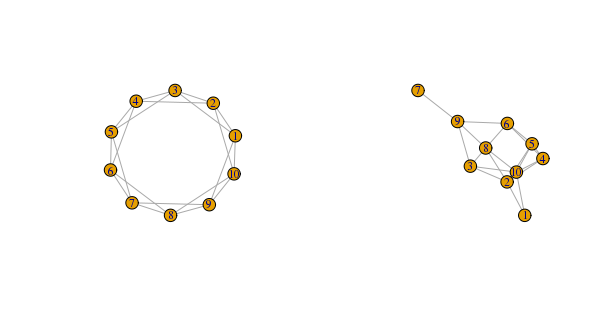
\includegraphics{figure/22wattsstrogatzexample.png}
  \caption{Examples of graphs generated from the Watts-Strogatz model.
  Both: \(N_V = 10\), \(r = 2\). Left: \(N_E = 20\). Right: \(N_E = 24\).}
  \end{figure}
  
  By adding edges, the diameter and average path length tend to decrease.
  This makes sense because this creates random shortcuts in the network
  framework. In the right-hand graph of Figure 2.2, which is the left-hand
  graph after adding \(4\) random
  edges--\(\{1, 5\}, \{2, 9\}, \{3, 10\}, \{4, 9\}\)--, we see that the
  diameter and average path length have decreased to \(2\), and \(1.467\),
  respectively.
  
  Like the Erdős-Rényi model, the Watts-Strogatz model also has very nice
  properties. Not only is it able to achieve a high clustering coefficient
  due to the inherent circular structure--which was definitely a drawback
  seen in the previous model--but adding in shortcuts also allow for
  average path lengths to be small as well. As we will see, this model has
  other properties, such as clustering coefficient, degree distribution,
  and triangle and triple counts.
  
  Given a circular model with \(N_{V}\) vertices and number of starting
  neighbors \(r\), a triangle on the model is represented by traveling
  across two edges in the same direction from a starting vertex, followed
  by one edge back to that vertex. With \(r\) neighbors, there are
  \({\frac {r} {2} \choose 2} = \frac {1} {4} N_{V} r \left(\frac {1} {2} r - 1 \right)\)
  ways to choose the two starting edges, and then \(N_V\) ways to take the
  last step back, making for a total of \(\frac {1} {2} N_{V} r(r - 1)\)
  triangles. The number of triples for each vertex is
  \({r \choose 2} = \frac {1} {2}r(r - 1)\) since any two unique edges
  from a vertex will connect three vertices. This, the total number of
  triples is \({r \choose 2} = \frac {1} {2}N_{V}r(r - 1)\).
  
  Combining these results, we have the clustering coefficient of the
  circular model. \[
  \begin{aligned}
  C &= \frac {(\text{number of pairs of neighbors of } i \text{ that are connected})} {(\text{number of pairs of neighbors of } i)} \\
  &= \frac {\frac {1} {4} N_{V} r \left(\frac {1} {2} r - 1 \right) \times 3} {\frac {1} {2} N_{V} r(r - 1)} \\
  &= \frac {3(r - 2)} {4(r - 1)}.
  \end{aligned}
  \] There is a minimum clustering coefficient of \(0\) if \(r = 2\) and a
  maximum of \(\frac {3} {4}\) as \(r \to \infty\). Note that this value
  is also independent of \(N_{V}\) (Newman 2010).
  
  The starting circular model has \(\frac {1} {2} N_{V}r\) non-shortcut
  edges. It is possible to add in shortcut edges to pairs of vertices that
  have yet to be connected with some probability \(p\). Thus, on average,
  we add approximately \(\frac {1} {2} N_{V}rp\) shortcuts--which mean
  there are \(N_{V}rp\) ends created by the shortcuts. The probability
  \(p_{s}\) that a number of shortcuts, \(s\), is attached to any one
  vertex has mean \(rp\) and follows a Poisson distribution
  \[p_{s} = e^{-rp} \frac {(rp)^{s}} {s!}.\] Using the fact that the total
  degree of a vertex \(k\) is the sum of the starting neighbors \(r\) and
  the number of starting shortcuts \(s\), that is \(k = r + s\), we can
  combine this with the equation above to get the degree distribution for
  the Watts-Strogaz model:
  
  \[p_{k} = e^{-rp} \frac {(rp)^{k - r}} {(k - r)!},\] for \(k \geq r\)
  and \(p_{k} = 0\) if \(k < r\) (Newman 2010).
  
  While it can be difficult to precisely calculate the clustering
  coefficient, we can calculate a limit for the number of triangles and
  triples. The number of triangles in the circular model remain unchanged,
  and the number of triangles created by the shortcuts is negligible
  compared to the number that the circle originally contained for large
  graphs. This is because the number of paths of length two that are
  completed by shortcuts to form triangles remains constant for large
  \(N_{V}\). The argument is similar for new triangles formed from two or
  three shortcuts as well. Thus, the leading term for the number of
  triangles in the Watts-Strogatz model is
  \(\frac {1} {4} N_{V}r \left(\frac {1} {2} r - 1 \right)\), which is
  equal to that of the circular model. For the number of triples, we
  consider the \(\frac {1} {2} N_{V} r(r - 1)\) triples from the circular
  structure itself, the \(\frac {1} {2}N_{V}rp\) shortcuts on average for
  each vertex times \(r\) neighbors times \(2\) ends for each shortcut
  equals \(N_{V}r^{2}p\) number of triples created by a shortcut combining
  with an edge in the circle, and the \(\frac {1} {2} r^{2} p^2\) expected
  number of connected triples centered at a vertex times \(N_{V}\)
  vertices equals \(\frac {1} {2} N_{V} r^{2} p^2\). Thus, \[
  \begin{aligned}
  C &= \frac {(\text{number of triangles}) \times 3} {\text{number of connected triples}}  \\
  &= \frac {\frac {1} {4} N_{V} r \left(\frac {1} {2} r - 1 \right) \times 3} {\frac {1} {2} N_{V} r(r - 1) + N_{V}r^{2}p + \frac {1} {2} N_{V} r^{2} p^2} \\
  &= \frac{3(r - 2)} {4(r - 1)+8rp + 4rp^{2}}.
  \end{aligned}
  \] When \(p = 0\), the clustering coefficient is equal to that of the
  circular model. And as \(p\) increases, the clustering coefficient will
  decrease. It reaches a minimum value of
  \(C = \frac {3(r - 2)} {(4c - 1)}\) when \(p = 1\) (Newman 2010).
  
  Calculating other parameters, such as average path length, are much more
  difficult for this model. In fact, no exact expressions for average path
  length have been discovered; only approximations. One special property
  of path lengths in this model, however, is that they \emph{scale} with
  the model parameters. This means that path length is calculated in terms
  of some function that does not depend on any parameters. For more
  information on scaling, see Newman (2010).
  
  While it is entirely possible that a network could potentially have some
  kind of rewiring process, it is less likely that this is true in the
  context of social networks. In other words, ties between people do not
  usually disappear and randomly reappear between others. However, we can
  still make use of the possibility that a social network can start with a
  circular model with some initial number of neighbors. New edges to
  create shortcuts can be added until we get a graph of similar order and
  size.
  
  In the case where we start with circular model of \(r = 1\) neighbor,
  however, this is no different from the Erdős-Rényi model. This is
  because the circular model with only one neighbor is very similar to a
  random assignment of edges (but with the restriction that each node only
  has a degree of \(1\)). Additionally, depending on the number of edges
  that need to be added to the network, the starting circle may not have a
  large effect on the overall structure of the graph generated.
  
  \section{Exponential Random Graph Models
  (ERGMs)}\label{exponential-random-graph-models-ergms}
  
  Exponential random graph models (ERGMs) are a class of models that can
  also be used to generate probability distributions for a set of random
  graphs. ERGMs have enormous flexibility in construction since they allow
  any combination of parameters from a given data set to be used in
  constructing the model. We are not only able to simulate additional
  graphs from the underlying probability distribution like in the
  Erdős-Rényi and Watts-Strogatz models, but we are also able to obtain
  maximum-likelihood estimates of the model for the data set and conduct
  goodness-of-fit tests for model assessment (Hunter et al. 2008a).
  
  The general form for an ERGM is as follows:
  \[P_{\theta, \mathcal{Y}}(\textbf{Y} = \textbf{y}) = \frac {exp(\theta^{T}\textbf{g(y)})} {\kappa(\theta, \mathcal{Y})},\textbf{y} \in \mathcal{Y}, \]
  where \(\textbf{Y}\) is the random variable representing the adjacency
  matrix of a graph and \(\textbf{y}\) is the particular adjacency matrix
  we observe. \(\textbf{g(y)}\) is the vector of model statistics for
  \(\textbf{y}\), \(\theta\) is the vector of coefficients for those
  statistics, and \(\kappa(\theta, \mathcal{Y})\) is the quantity in the
  numerator summed over all possible networks. The
  \(\theta^{T}\textbf{g(y)}\) is a polynomial of coefficients \(\theta\)
  and statistics \(g(y)\). This statistics could be things such as the
  number of edges or triangles of a graph in question. The \(\theta\)
  parameters are interpreted as the log odds of an individual tie
  conditional on all the others (Hunter et al. 2008a, Butts et al. 2015,
  Jackson 2013).
  
  The denominator
  \[\kappa(\theta, \mathcal{Y}) = \sum_{z \in \mathcal{Y}}^{} exp(\theta^{T}\textbf{g(y)})\]
  serves as a normalizing factor so that
  \(P_{\theta, \mathcal{Y}}(\textbf{Y} = \textbf{y})\) is a proper
  probability distribution (that is, the values that are output are
  between \(0\) and \(1\)). It is also possible to consider actual graphs
  themselves instead of their adjacency matrices. This means we can
  replace \(\textbf{y}\) with an observed graph \(g\), \(\textbf{Y}\) with
  a random graph \(G\), and \(\mathcal{Y}\) with the ensemble of graphs
  \(\mathcal{G}\).
  
  As an example, consider a graph \(g\) with the following statistics:
  \(L(g)\) is the number of edges in the graph, \(T(g)\) is the number of
  triangles, and \(K(g)\) is the number of k-stars.
  
  Using an ERGM to fit \(g\) would result in the following probability
  distribution:
  \[P_{\theta, \mathcal{G}}(g) = \frac {exp(\theta_{L}L(g) + \theta_{T}T(g)+\theta_{K}K(g))} {\sum_{g' \in \mathcal{G}}^{} exp(\theta_{L}L(g) + \theta_{T}T(g)+\theta_{K}K(g))}, g \in \mathcal{G}.\]
  
  The statistics used to build an ERGM are either \emph{dyad independent}
  or \emph{dyad dependent} terms (\emph{dyad} meaning \emph{edge}). Dyad
  independent terms (such as edges between nodes, \(L(g)\)) imply no
  dependence between the edges of other nodes. Thus, the presence or
  absence of an edge between vertices does not affect and is not affected
  by the presence and absence of other edges. On the other hand, dyad
  dependent terms (such as triangles, \(T(g)\) and k-stars \(K(g)\)) do
  imply dependence among edges in the graph; the absence of a link does
  affect the triangle and k-star counts. In order to calculate the
  \(\theta\) parameters, ERGMs implement an estimation algorithm. If the
  model only contains dyad independent terms, the algorithm is simply a
  maximum log-likelihood estimation, in which we find the value that
  maximizes the log-probability model. However, if the ERGM contains dyad
  dependent terms, it can be impossible to obtain a closed form of the
  probability model and estimate the parameters by maximizing the
  log-likelihood function. Instead, we turn to a new method of estimation,
  called \emph{Markov chain Monte Carlo (MCMC)}. In short, this means we
  estimate the parameters via simulation rather than precise calculation
  (Butts et al. 2015). See Gilks, Richardson, \& Spiegelhalter (1995) for
  more information about MCMC.
  
  \subsection{Deriving the Erdős-Rényi Model from
  ERGMs}\label{deriving-the-erdos-renyi-model-from-ergms}
  
  The Erdős-Rényi and Watts-Strogatz models are actually special cases of
  ERGMs. Here, we will show that the Erdős-Rényi model can be derived from
  an ERGM that only takes into acount the number of edges in a graph.
  Suppose we have a particular graph \(g\) and the only statistic we have
  is \(L(G)\), the number of edges in \(g\). Our probability model is thus
  \[P_{\theta, \mathcal{G}}(g) = \frac {exp(\theta_{L}L(g))} {\sum_{g' \in \mathcal{G}}^{} exp(\theta_{L}L(g'))}, g \in \mathcal{G}.\]
  
  Consider the probability distribution for a particular graph \(g\) with
  \(N_E\) edges again (from the Erdős-Rényi model). Using the fact that
  \(N_{E} = L(g)\), taking the equation as a power of base \(e\), we get
  the following: \[
  \begin{aligned}
  P(g) &= p^{N_E}(1 - p)^{\left({N_V \choose 2} - N_E \right)} \\
  &= p^{L(g)}(1 - p)^{\left(\frac {N_{V}(N_{V} - 1)} {2} - L(g) \right)} \\
  &= \left( \frac {p} {1-p} \right)^{L(g)}(1 - p)^{\frac {N_{V}(N_{V} - 1)} {2}} \\
  &= exp \left(L(g)log \left(\frac {p} {1-p} \right) - \frac {N_{V}(N_{V} - 1)} {2} log \left( \frac {p} {1-p} \right) \right) \\
  &= exp(\theta_{L}L(g) - c) \\
  &= \frac {exp(\theta_{L}L(g))} {exp(c)},
  \end{aligned} 
  \] where
  \(c = \frac {N_{V}(N_{V} - 1)} {2} ln \left( \frac {p} {1-p} \right)\)
  is the normalizing constant \(\kappa(\theta, \mathcal{Y})\) seen in the
  general form of an ERGM and exactly the denominator
  \(\sum_{g' \in \mathcal{G}}^{} exp(\theta_{L}L(g'))\) seen in the ERGM
  that fits a graph \(g\) with only the edge statistic \(L(g)\) (Hunter et
  al. 2008a \& Jackson 2013).
  
  \chapter{Simulation Study}\label{simulation-study}
  
  We will use a subset of the Facebook network for our analysis. We fit
  graph models to the observed network and assess each model's accuracy by
  comparing the network statistics of the observed network to the graphs
  generated by the models.
  
  \section{Description of the Dataset}\label{description-of-the-dataset}
  
  This Facebook network was compiled by Stanford University and was
  accessed through the Stanford Large Network Data Collection (SNAP). For
  more information, please see Jure Leskovec \& Krevl (2014). Our subset
  of the Facebook network was presented as an edge list. The social
  network is one giant component composed of \(4039\) vertices and
  \(88234\) edges, which represent \(4039\) anonymous users and the
  \(88234\) connections between them, respectively.\footnote{Some of our
    network statistics that we calculated in R did not match those shown
    in the SNAP website. For example, we calculated the diameter and
    transitivity of this Facebook component to be \(17\) and \(0.617\),
    respectively. However, the SNAP website reports the diameter and
    ``average clustering coefficient'' to be \(8\) and \(0.6055\),
    respectively. However, other values, such as vertex and edge count, as
    well as the number of triangles, are equal. While SNAP's algorithm
    used to calculate their network statistics is unclear, for the
    purposes of this simulation study, we will be using the values that we
    calculated from the Facebook component to compare with those generated
    from our graph models.} This network is simple and undirected, and we
  believe that the network consists of established, mutual friendships.
  The first column of values in Table 3.1 below describes some
  characteristics of this network. We use the \texttt{igraph},
  \texttt{sna}, \texttt{network}, \texttt{ergm}, and \texttt{statnet}
  packages in this study.\footnote{See Csárdi \& Nepusz (2006), C. T.
    Butts \& others (2008), Butts (2015), Butts (2008), Handcock et al.
    (2017), David R. Hunter et al. (2008b), Handcock et al. (2016),
    Handcock, Hunter, Butts, Goodreau, \& Morris (2008b), and Bojanowski
    (2015) for more details about these packages.}
  
  \begin{figure}[htbp]
  \centering
  \includegraphics{figure/31fbelplot.pdf}
  \caption{Overview of our component of the Facebook network}
  \end{figure}
  
  \section{Generating Random Graphs}\label{generating-random-graphs}
  
  For each model, we create graphs of parable magnitude using some of the
  information calculated from the our Facebook network. We compare
  selected statistical network statistics of the Facebook network with
  that of the graphs we generate to see if the observed network and the
  simulated graphs have similar characteristics. In the sections below, we
  explain the algorithm, or steps, to simulate one random graph for each
  model in the sections below. We simulate \(1000\) random graphs for each
  model and record the statistics such as transitivity, diameter, and
  average centrality values. Because we have \(1000\) values--one for each
  random graph for each model--we can obtain a distribution of these
  values or a table of average values.
  
  \subsection{Using the Erdős-Rényi
  Model}\label{using-the-erdos-renyi-model}
  
  Recall that the Erdős-Rényi model takes in only two parameters, which
  are the number of vertices, \(N_{V}\), and the fixed probability of edge
  forming between any two different vertices, \(p\). The number of
  vertices is already given as \(4039\), but to find the probability, we
  estimate this by taking the number of observed edges and dividing it by
  the number of possible edges. For a graph \(G\), this estimated
  probability, \(\hat{p}\), is
  \[\hat{p} = \frac {N_{E}} {{N_{V} \choose 2}},\] where \(N_{E}\) is the
  number of edges in \(G\) and \(N_{V}\) is the number of vertices in
  \(G\). Our estimated probability \(\hat{p}\) for this Facebook network
  is then \(\frac {88234} {{4039 \choose 2}}\), or approximately
  \(0.011\). Thus, in order to simulate one graph from this model, we must
  look at every possible edge among the \(4039\) vertices and determine if
  an edge will form based on the given probability.
  
  \subsection{Using the Watts-Strogatz
  Model}\label{using-the-watts-strogatz-model}
  
  Recall that the Watts-Strogatz model takes in the following parameters:
  the number of vertices \(N_{V}\), the number of starting neighbors
  \(r\), and the probability of an edge to be rewired \(p\). However,
  instead of rewiring our edges with a fixed probability, we will instead
  randomly add edges until we have approximately the same number as our
  observed network. To do this, we start with a lattice with \(4039\)
  vertices and assign a number of edges to the vertices equal to the
  smallest degree seen in our Facebook network (which we find to be
  \(1\)). This is our starting number of neighbors for each vertex. In
  this situation, \(p = 0\). We then randomly add edges equal to the
  difference between the our starting lattice and the observed network.
  That is, we add \(88234 - 4039 = 84195\) edges to our lattice. Finally,
  we simplify our simulated graph to eliminate multi-edges and loops.
  Since there are \(4039 \choose 2\) edges to choose from, intuitively, we
  can see that having many multi-edges or loops will be infrequent. This
  makes up one simulated graph from the model.
  
  \subsection{Using ERGMs}\label{using-ergms}
  
  We consider four different ERGMs--which we label as ERGM 1a, ERGM 2a,
  ERGM 2b, and ERGM 3a. ERGM 1a takes in only the most basic parameter:
  edges. In Chapter 2, we have already shown its relationship to the
  Erdős-Rényi model. ERGM 2a and 2b both take in two parameters: edges and
  triangles for 2a, and edges and k-stars (of size 3) for 2b. Lastly, ERGM
  3a, takes in all three parameters: edges, triangles, and k-stars (of
  size 3). Similar to linear regression, adding in more parameters will
  allow the ERGM to fit more closely to the observed network but at the
  cost of greater complexity. We do not consider models that only consist
  of just the triangle parameter or just the k-star parameter. This is
  because information about k-stars and triangles are based on some
  knowledge about edges anyway. After fitting ERGMs with the desired
  parameters (via maximum likelihood or MCMC), we begin simulating random
  graphs from each model. For each random graph, we calculate the networks
  statistics of interest to us.
  
  \clearpage
  
  \begin{longtable}[]{@{}lccc@{}}
  \caption{Comparisons of network statistics among graphs simulated from
  the Erdős-Rényi and Watts-Strogatz models and the observed network
  (estimate \(\pm\) standard deviation)
  \label{tab:erwsdescstats}}\tabularnewline
  \toprule
  \begin{minipage}[b]{0.18\columnwidth}\raggedright\strut
  Network Statistic\strut
  \end{minipage} & \begin{minipage}[b]{0.13\columnwidth}\centering\strut
  Observed\strut
  \end{minipage} & \begin{minipage}[b]{0.29\columnwidth}\centering\strut
  Erdős-Rényi\strut
  \end{minipage} & \begin{minipage}[b]{0.29\columnwidth}\centering\strut
  Watts-Strogatz\strut
  \end{minipage}\tabularnewline
  \midrule
  \endfirsthead
  \toprule
  \begin{minipage}[b]{0.18\columnwidth}\raggedright\strut
  Network Statistic\strut
  \end{minipage} & \begin{minipage}[b]{0.13\columnwidth}\centering\strut
  Observed\strut
  \end{minipage} & \begin{minipage}[b]{0.29\columnwidth}\centering\strut
  Erdős-Rényi\strut
  \end{minipage} & \begin{minipage}[b]{0.29\columnwidth}\centering\strut
  Watts-Strogatz\strut
  \end{minipage}\tabularnewline
  \midrule
  \endhead
  \begin{minipage}[t]{0.18\columnwidth}\raggedright\strut
  Transitivity\strut
  \end{minipage} & \begin{minipage}[t]{0.13\columnwidth}\centering\strut
  0.617\strut
  \end{minipage} & \begin{minipage}[t]{0.29\columnwidth}\centering\strut
  0.0108 \(\pm\) 0.0001\strut
  \end{minipage} & \begin{minipage}[t]{0.29\columnwidth}\centering\strut
  0.0107 \(\pm\) 9e-05\strut
  \end{minipage}\tabularnewline
  \begin{minipage}[t]{0.18\columnwidth}\raggedright\strut
  Avg. Path Length\strut
  \end{minipage} & \begin{minipage}[t]{0.13\columnwidth}\centering\strut
  4.338\strut
  \end{minipage} & \begin{minipage}[t]{0.29\columnwidth}\centering\strut
  2.606 \(\pm\) 0.002\strut
  \end{minipage} & \begin{minipage}[t]{0.29\columnwidth}\centering\strut
  2.609 \(\pm\) 0.0002\strut
  \end{minipage}\tabularnewline
  \begin{minipage}[t]{0.18\columnwidth}\raggedright\strut
  Diameter\strut
  \end{minipage} & \begin{minipage}[t]{0.13\columnwidth}\centering\strut
  17\strut
  \end{minipage} & \begin{minipage}[t]{0.29\columnwidth}\centering\strut
  3.96 \(\pm\) 0.21\strut
  \end{minipage} & \begin{minipage}[t]{0.29\columnwidth}\centering\strut
  3.95 \(\pm\) 0.22\strut
  \end{minipage}\tabularnewline
  \begin{minipage}[t]{0.18\columnwidth}\raggedright\strut
  Degree Cen.\strut
  \end{minipage} & \begin{minipage}[t]{0.13\columnwidth}\centering\strut
  43.69\strut
  \end{minipage} & \begin{minipage}[t]{0.29\columnwidth}\centering\strut
  43.69 \(\pm\) 0.14\strut
  \end{minipage} & \begin{minipage}[t]{0.29\columnwidth}\centering\strut
  43.45 \(\pm\) 0.01\strut
  \end{minipage}\tabularnewline
  \begin{minipage}[t]{0.18\columnwidth}\raggedright\strut
  Betweenness Cen.\strut
  \end{minipage} & \begin{minipage}[t]{0.13\columnwidth}\centering\strut
  2072.642\strut
  \end{minipage} & \begin{minipage}[t]{0.29\columnwidth}\centering\strut
  3242 \(\pm\) 4\strut
  \end{minipage} & \begin{minipage}[t]{0.29\columnwidth}\centering\strut
  3249.2 \(\pm\) 0.4\strut
  \end{minipage}\tabularnewline
  \begin{minipage}[t]{0.18\columnwidth}\raggedright\strut
  Closeness Cen.\strut
  \end{minipage} & \begin{minipage}[t]{0.13\columnwidth}\centering\strut
  8.88e-08\strut
  \end{minipage} & \begin{minipage}[t]{0.29\columnwidth}\centering\strut
  9.507e-05 \(\pm\) 7e-08\strut
  \end{minipage} & \begin{minipage}[t]{0.29\columnwidth}\centering\strut
  9.494e-05 \(\pm\) 7e-09\strut
  \end{minipage}\tabularnewline
  \begin{minipage}[t]{0.18\columnwidth}\raggedright\strut
  Eigenvector Cen.\strut
  \end{minipage} & \begin{minipage}[t]{0.13\columnwidth}\centering\strut
  0.040\strut
  \end{minipage} & \begin{minipage}[t]{0.29\columnwidth}\centering\strut
  0.620 \(\pm\) 0.022\strut
  \end{minipage} & \begin{minipage}[t]{0.29\columnwidth}\centering\strut
  0.6235 \(\pm\) 0.0227\strut
  \end{minipage}\tabularnewline
  \bottomrule
  \end{longtable}
  
  \begin{longtable}[]{@{}lccc@{}}
  \caption{Comparisons of network statistics among graphs simulated from
  ERGMs (1a: edges and 2a: edges and triangles) and the observed network
  (estimate \(\pm\) standard deviation)
  \label{tab:ergm1a2a}}\tabularnewline
  \toprule
  \begin{minipage}[b]{0.20\columnwidth}\raggedright\strut
  Network Statistic\strut
  \end{minipage} & \begin{minipage}[b]{0.12\columnwidth}\centering\strut
  Observed\strut
  \end{minipage} & \begin{minipage}[b]{0.27\columnwidth}\centering\strut
  ERGM1a\strut
  \end{minipage} & \begin{minipage}[b]{0.29\columnwidth}\centering\strut
  ERGM2a\strut
  \end{minipage}\tabularnewline
  \midrule
  \endfirsthead
  \toprule
  \begin{minipage}[b]{0.20\columnwidth}\raggedright\strut
  Network Statistic\strut
  \end{minipage} & \begin{minipage}[b]{0.12\columnwidth}\centering\strut
  Observed\strut
  \end{minipage} & \begin{minipage}[b]{0.27\columnwidth}\centering\strut
  ERGM1a\strut
  \end{minipage} & \begin{minipage}[b]{0.29\columnwidth}\centering\strut
  ERGM2a\strut
  \end{minipage}\tabularnewline
  \midrule
  \endhead
  \begin{minipage}[t]{0.20\columnwidth}\raggedright\strut
  Transitivity\strut
  \end{minipage} & \begin{minipage}[t]{0.12\columnwidth}\centering\strut
  0.617\strut
  \end{minipage} & \begin{minipage}[t]{0.27\columnwidth}\centering\strut
  0.3696 \(\pm\) 0.0012\strut
  \end{minipage} & \begin{minipage}[t]{0.29\columnwidth}\centering\strut
  0.4823 \(\pm\) 0.0020\strut
  \end{minipage}\tabularnewline
  \begin{minipage}[t]{0.20\columnwidth}\raggedright\strut
  Avg. Path Length\strut
  \end{minipage} & \begin{minipage}[t]{0.12\columnwidth}\centering\strut
  4.338\strut
  \end{minipage} & \begin{minipage}[t]{0.27\columnwidth}\centering\strut
  2.885 \(\pm\) 0.004\strut
  \end{minipage} & \begin{minipage}[t]{0.29\columnwidth}\centering\strut
  3.052 \(\pm\) 0.009\strut
  \end{minipage}\tabularnewline
  \begin{minipage}[t]{0.20\columnwidth}\raggedright\strut
  Diameter\strut
  \end{minipage} & \begin{minipage}[t]{0.12\columnwidth}\centering\strut
  17\strut
  \end{minipage} & \begin{minipage}[t]{0.27\columnwidth}\centering\strut
  5.216 \(\pm\) 0.412\strut
  \end{minipage} & \begin{minipage}[t]{0.29\columnwidth}\centering\strut
  6.098 \(\pm\) 0.035\strut
  \end{minipage}\tabularnewline
  \begin{minipage}[t]{0.20\columnwidth}\raggedright\strut
  Degree Cen.\strut
  \end{minipage} & \begin{minipage}[t]{0.12\columnwidth}\centering\strut
  43.69\strut
  \end{minipage} & \begin{minipage}[t]{0.27\columnwidth}\centering\strut
  43.66 \(\pm\) 0.05\strut
  \end{minipage} & \begin{minipage}[t]{0.29\columnwidth}\centering\strut
  44.54 \(\pm\) 0.03\strut
  \end{minipage}\tabularnewline
  \begin{minipage}[t]{0.20\columnwidth}\raggedright\strut
  Betweenness Cen.\strut
  \end{minipage} & \begin{minipage}[t]{0.12\columnwidth}\centering\strut
  2072.642\strut
  \end{minipage} & \begin{minipage}[t]{0.27\columnwidth}\centering\strut
  3805 \(\pm\) 9\strut
  \end{minipage} & \begin{minipage}[t]{0.29\columnwidth}\centering\strut
  4140 \(\pm\) 18\strut
  \end{minipage}\tabularnewline
  \begin{minipage}[t]{0.20\columnwidth}\raggedright\strut
  Closeness Cen.\strut
  \end{minipage} & \begin{minipage}[t]{0.12\columnwidth}\centering\strut
  8.88e-08\strut
  \end{minipage} & \begin{minipage}[t]{0.27\columnwidth}\centering\strut
  8.286e-05 \(\pm\) 8.35e-06\strut
  \end{minipage} & \begin{minipage}[t]{0.29\columnwidth}\centering\strut
  6.01e-05 \(\pm\) 1.51e-05\strut
  \end{minipage}\tabularnewline
  \begin{minipage}[t]{0.20\columnwidth}\raggedright\strut
  Eigenvector Cen.\strut
  \end{minipage} & \begin{minipage}[t]{0.12\columnwidth}\centering\strut
  0.040\strut
  \end{minipage} & \begin{minipage}[t]{0.27\columnwidth}\centering\strut
  0.0417 \(\pm\) 0.0008\strut
  \end{minipage} & \begin{minipage}[t]{0.29\columnwidth}\centering\strut
  0.041 \(\pm\) 5e-05\strut
  \end{minipage}\tabularnewline
  \bottomrule
  \end{longtable}
  
  \begin{longtable}[]{@{}lccc@{}}
  \caption{Comparisons of network statistics among graphs simulated from
  ERGMs (2b: edges and k-stars(\(3\)) and 3a: edges, triangles, and
  k-stars(\(3\))) and the observed network (estimate \(\pm\) standard
  deviation) \label{tab:ergm2b3a}}\tabularnewline
  \toprule
  \begin{minipage}[b]{0.20\columnwidth}\raggedright\strut
  Network Statistic\strut
  \end{minipage} & \begin{minipage}[b]{0.12\columnwidth}\centering\strut
  Observed\strut
  \end{minipage} & \begin{minipage}[b]{0.27\columnwidth}\centering\strut
  ERGM2b\strut
  \end{minipage} & \begin{minipage}[b]{0.29\columnwidth}\centering\strut
  ERGM3a\strut
  \end{minipage}\tabularnewline
  \midrule
  \endfirsthead
  \toprule
  \begin{minipage}[b]{0.20\columnwidth}\raggedright\strut
  Network Statistic\strut
  \end{minipage} & \begin{minipage}[b]{0.12\columnwidth}\centering\strut
  Observed\strut
  \end{minipage} & \begin{minipage}[b]{0.27\columnwidth}\centering\strut
  ERGM2b\strut
  \end{minipage} & \begin{minipage}[b]{0.29\columnwidth}\centering\strut
  ERGM3a\strut
  \end{minipage}\tabularnewline
  \midrule
  \endhead
  \begin{minipage}[t]{0.20\columnwidth}\raggedright\strut
  Transitivity\strut
  \end{minipage} & \begin{minipage}[t]{0.12\columnwidth}\centering\strut
  0.617\strut
  \end{minipage} & \begin{minipage}[t]{0.27\columnwidth}\centering\strut
  0.379 \(\pm\) 0.001\strut
  \end{minipage} & \begin{minipage}[t]{0.29\columnwidth}\centering\strut
  0.489 \(\pm\) 0.002\strut
  \end{minipage}\tabularnewline
  \begin{minipage}[t]{0.20\columnwidth}\raggedright\strut
  Avg. Path Length\strut
  \end{minipage} & \begin{minipage}[t]{0.12\columnwidth}\centering\strut
  4.338\strut
  \end{minipage} & \begin{minipage}[t]{0.27\columnwidth}\centering\strut
  2.851 \(\pm\) 0.003\strut
  \end{minipage} & \begin{minipage}[t]{0.29\columnwidth}\centering\strut
  3.056 \(\pm\) 0.008\strut
  \end{minipage}\tabularnewline
  \begin{minipage}[t]{0.20\columnwidth}\raggedright\strut
  Diameter\strut
  \end{minipage} & \begin{minipage}[t]{0.12\columnwidth}\centering\strut
  17\strut
  \end{minipage} & \begin{minipage}[t]{0.27\columnwidth}\centering\strut
  5.095 \(\pm\) 0.293\strut
  \end{minipage} & \begin{minipage}[t]{0.29\columnwidth}\centering\strut
  6.161 \(\pm\) 0.368\strut
  \end{minipage}\tabularnewline
  \begin{minipage}[t]{0.20\columnwidth}\raggedright\strut
  Degree Cen.\strut
  \end{minipage} & \begin{minipage}[t]{0.12\columnwidth}\centering\strut
  43.69\strut
  \end{minipage} & \begin{minipage}[t]{0.27\columnwidth}\centering\strut
  44.06 \(\pm\) 0.06\strut
  \end{minipage} & \begin{minipage}[t]{0.29\columnwidth}\centering\strut
  44.52 \(\pm\) 0.03\strut
  \end{minipage}\tabularnewline
  \begin{minipage}[t]{0.20\columnwidth}\raggedright\strut
  Betweenness Cen.\strut
  \end{minipage} & \begin{minipage}[t]{0.12\columnwidth}\centering\strut
  2072.642\strut
  \end{minipage} & \begin{minipage}[t]{0.27\columnwidth}\centering\strut
  3736 \(\pm\) 6\strut
  \end{minipage} & \begin{minipage}[t]{0.29\columnwidth}\centering\strut
  4148 \(\pm\) 16\strut
  \end{minipage}\tabularnewline
  \begin{minipage}[t]{0.20\columnwidth}\raggedright\strut
  Closeness Cen.\strut
  \end{minipage} & \begin{minipage}[t]{0.12\columnwidth}\centering\strut
  8.88e-08\strut
  \end{minipage} & \begin{minipage}[t]{0.27\columnwidth}\centering\strut
  8.558e-05 \(\pm\) 6.03e-06\strut
  \end{minipage} & \begin{minipage}[t]{0.29\columnwidth}\centering\strut
  5.88e-05 \(\pm\) 1.50e-05\strut
  \end{minipage}\tabularnewline
  \begin{minipage}[t]{0.20\columnwidth}\raggedright\strut
  Eigenvector Cen.\strut
  \end{minipage} & \begin{minipage}[t]{0.12\columnwidth}\centering\strut
  0.040\strut
  \end{minipage} & \begin{minipage}[t]{0.27\columnwidth}\centering\strut
  0.0392 \(\pm\) 0.0002\strut
  \end{minipage} & \begin{minipage}[t]{0.29\columnwidth}\centering\strut
  0.0410 \(\pm\) 3e-05\strut
  \end{minipage}\tabularnewline
  \bottomrule
  \end{longtable}
  
  The first column of \autoref{tab:erwsdescstats}, \autoref{tab:ergm1a2a},
  and \autoref{tab:ergm2b3a} shows the network statistics we are
  interested in. The second column of each table lists the true value of
  the statistis associated with the Facebook component. Each of the other
  cells contain an estimated network statistic and standard deviation
  under each model. For statistics such as average degree, we were
  interested in recording an average of the average values. Additionally,
  because each simulated graph will have approximately the same number of
  vertices, we, again, do not scale these values.
  
  Based on \autoref{tab:erwsdescstats}, we see that the estimated average
  statistics for the Erdős-Rényi and Watts-Strogatz models are very
  similar to each other but are drastically different from many of the
  observed values of our Facebook network. This means that while the
  graphs generated from each model look very similar to each other, they
  look drastically different from our observed Facebook network. This
  comes as no surprise since the methods used to construct graphs under
  both models are very likely to generate almost the same number of
  vertices. We even see this in our simulation study; in the fourth row of
  \autoref{tab:erwsdescstats}, the average degree estimate for both models
  was within one degree of the other. Additionally, in both constructions,
  we are adding the edges randomly, so they are almost always spread
  evenly throughout the \(4039\) vertices. This means that additional
  features of the observed network, such as large clusters or degrees with
  high centralities, are likely to be missed by graphs generated from
  these two models. This is why the transitivity, average path length, and
  diameter for both models are much smaller than what was actually
  observed.
  
  Similarly, due to the random disperal of edges throughout the network,
  there is little control in deciding which vertices and how many are
  considered important, making the average centrality measures for the
  random graphs much larger than those seen in the observed model. The
  only statistic whose value was actually close to, if not equal to, the
  observed value was the average degree. However, this makes sense since
  we fixed the probability \(p\) of a link forming in the Erdős-Rényi
  model (which is directly proportional to the average degree) and because
  we ensured that every graph generated from the Watts-Strogatz model has
  about the same number of edges as the observed network. Thus, we have
  shown through this simulation study that the Erdős-Rényi and
  Watts-Strogatz models are not very accurate in modeling our Facebook
  network for these particular network statistics.
  
  As \autoref{tab:ergm1a2a} and \autoref{tab:ergm2b3a} suggest, it appears
  that the random graphs generated from ERGMs provide very good estimates
  of average degree and average eigenvector centrality. Estimates of other
  network statistics, however, are quite different from what is actually
  observed. Not surprisingly, many of the average network statistics of
  the random graphs generated by the ERGMs get closer to the observed
  value as the number of parameters increase. This includes an overall
  increase in transitivity, average path length, and diameter and an
  overall decrease of average closeness centrality as the number of
  parameters increase from one to three. Average betweenness centrality,
  however, continues to drift farther away from the observed value as the
  number of parameters increase.
  
  The fact that ERGM 2a (edges and triangles) has such similar values to
  ERGM 3a (edges, triangles, and k-stars of size \(3\)) in spite the
  difference in the number of parameters suggests that the k-star
  parameter may be redundant. This is also further suggested by the fact
  that ERGM 2b (edges and k-stars of size \(3\)) and ERGM 1a (edges) are
  also very similar in values as well. While this simulation study
  suggests that the right combinations of parameters could potentially
  allow for an ERGM to accurately model an observed network, we conclude
  that the four ERGMs used in this study do not do a very good job of
  modeling our Facebook network for these particular network statistics.
  
  \chapter{Conclusion}\label{conclusion}
  
  In this thesis, we have provided a brief overview of networks, including
  network statistics and some graph models. We also applied certain graph
  models--such as the Erdős-Rényi and Watts-Strogatz models along with
  various ERGMs with different combinations of parameters--and fitted them
  to our component of the Facebook network. By letting the graph models
  take in certain parameters of our Facebook network, we generated graphs
  of parable magnitude. We compared the network statistics between these
  generated graphs and our target network to measure each model's
  accuracy. This simulation study suggested that none of the models that
  we examined did a good job of modeling the Facebook network for our
  chosen network statistics.
  
  However, this simulation study only scratches the surface of what
  network science has to offer. Firstly, we can simply change our approach
  with Erdős-Rényi, Watts-Strogatz, and exponential random graph models we
  have so far. In applying the Erdős-Rényi model, we had used the
  \(G(N_{V}, p)\) model. For the same of comparison, we could also explore
  how well the \(G(N_{V}, N_{E})\) model fits the Facebook network. Our
  use of the Watts-Strogatz model began with a circular lattice with only
  one neighbor. Instead of specifying a probability \(p\) of a shortcut
  forming, we simply added ``enough'' edges so that they are similar to
  the observed Facebook network. While the methodology is logical, the
  results of the simulation study become very similar to that of the
  Erdős-Rényi model and we ultimately lose the characteristic of high
  transitivity that the Watts-Strogatz model is known for. Future
  applications of the Watts-Strogatz model should include a logical
  methodology to make better use of the circular model and shortcut
  probability \(p\). ERGMs seemed to have the most promise--as we increase
  the number of parameters, we see that the estimates of many network
  statistics tend to approach the observed value. This suggests that
  trying other ERGMs with more parameters and different combinations of
  them could potentially improve the results of this study. See C. Butts
  et al. (2015) for a list of possible ERGM parameters to choose from.
  
  Additionally, we can bring in other social networks into this study.
  Could underlying undirected graphs of directed networks be a better fit
  for the models here? We could potentially analyze a different dataset,
  such as Twitter, in which we look at the underlying graph of directed
  followers instead of mutual friendships. Could network size be a factor
  as well? The Facebook component we are currently observing could perhaps
  be too small and cause issues of variance. It is also possible for us to
  test other network statistics. Without providing the definitions, we can
  consider values such as \emph{reciprocity}, \emph{assortativity}, or
  even other kinds of centrality measures. See Newman (2010) for more
  details.
  
  It is also possible for us to choose other models to test our current
  Facebook network on. In fact, many other graphs models exist beyond what
  was presented here. Because social networks exhibit certain
  characteristics different from other kinds of networks, it comes as no
  surprise that there have been other models that are specifically
  tailored to its study. See Toivonen et al. (2009) for a study of
  \emph{network evolution models} and \emph{nodal attribute models}, two
  specific types of social network models. Also, see Jurij Leskovec,
  Chakrabarti, Kleinberg, \& Faloutsos (2005) and Jure Leskovec,
  Chakrabarti, Kleinberg, Faloutsos, \& Ghahramani (2010) about more
  recent developments in network science. They introduce models called
  \emph{Kronecker graphs} that have the benefit of only requiring a few
  parameters to fit to a target network in linear time.
  
  A successful simulation study has many implications and can benefit not
  only statistics and network science, but in just about all other
  disciplines as well.
  
  \singlespacing
  \appendix
  
  \chapter{R/R-Markdown Code}\label{rr-markdown-code}
  
  This first appendix includes all of the R chunks of code used throughout
  the document (using the \texttt{include\ =\ FALSE} chunk tag) to help
  with readability and/or setup. Some code chunks were shown in the main
  body of the chapters for clarity and illustration.
  
  \subsubsection{In the main Rmd file:}\label{in-the-main-rmd-file}
  
  This is the setup file for the template.
  
  \begin{Shaded}
  \begin{Highlighting}[]
  \CommentTok{# This chunk ensures that the acstats package is}
  \CommentTok{# installed and loaded. This acstats package includes}
  \CommentTok{# the template files for the thesis and also two functions}
  \CommentTok{# used for labeling and referencing}
  \NormalTok{if(!}\KeywordTok{require}\NormalTok{(devtools))}
    \KeywordTok{install.packages}\NormalTok{(}\StringTok{"devtools"}\NormalTok{, }\DataTypeTok{repos =} \StringTok{"http://cran.rstudio.com"}\NormalTok{)}
  \NormalTok{if(!}\KeywordTok{require}\NormalTok{(acstats))\{}
    \KeywordTok{library}\NormalTok{(devtools)}
    \NormalTok{devtools::}\KeywordTok{install_github}\NormalTok{(}\StringTok{"Amherst-Statistics/acstats"}\NormalTok{)}
  \NormalTok{\}}
  \KeywordTok{library}\NormalTok{(acstats)}
  \end{Highlighting}
  \end{Shaded}
  
  The following are the packages used throughout this work. In particular,
  the \texttt{igraph}, \texttt{network}, \texttt{statnet}, and
  \texttt{ergm} packages were heavily used throughout all the chapters.
  
  \begin{Shaded}
  \begin{Highlighting}[]
  \KeywordTok{library}\NormalTok{(sand)}
  \KeywordTok{library}\NormalTok{(igraph)}
  \KeywordTok{library}\NormalTok{(network)}
  \KeywordTok{library}\NormalTok{(sna)}
  \KeywordTok{library}\NormalTok{(statnet)}
  \KeywordTok{library}\NormalTok{(ergm)}
  \KeywordTok{library}\NormalTok{(xtable)}
  
  \KeywordTok{options}\NormalTok{(}\DataTypeTok{xtable.comment =} \OtherTok{FALSE}\NormalTok{)}
  \KeywordTok{options}\NormalTok{(}\DataTypeTok{digits =} \DecValTok{4}\NormalTok{)}
  \end{Highlighting}
  \end{Shaded}
  
  \subsubsection{In Introduction}\label{in-introduction}
  
  We use the \texttt{karate} and \texttt{lawyer} data sets as examples to
  illustrate our discussion of networks.
  
  \begin{Shaded}
  \begin{Highlighting}[]
  \KeywordTok{data}\NormalTok{(karate)}
  \KeywordTok{data}\NormalTok{(lazega)}
  \end{Highlighting}
  \end{Shaded}
  
  The following code chunk generates a visual representing Zachary's
  karate club network. See Figure 1.
  
  \begin{Shaded}
  \begin{Highlighting}[]
  \KeywordTok{plot}\NormalTok{(karate)}
  \end{Highlighting}
  \end{Shaded}
  
  The following code chunk generates a visual representing Lazega's law
  firm network. See Figure 2.
  
  \begin{Shaded}
  \begin{Highlighting}[]
  \CommentTok{# Office location indicated by color.}
  \NormalTok{colbar <-}\StringTok{ }\KeywordTok{c}\NormalTok{(}\StringTok{"red"}\NormalTok{, }\StringTok{"dodgerblue"}\NormalTok{, }\StringTok{"goldenrod"}\NormalTok{)}
  \NormalTok{v.colors <-}\StringTok{ }\NormalTok{colbar[}\KeywordTok{V}\NormalTok{(lazega)$Office]}
  \CommentTok{# Type of practice indicated by vertex shape.}
  \NormalTok{v.shapes <-}\StringTok{ }\KeywordTok{c}\NormalTok{(}\StringTok{"circle"}\NormalTok{, }\StringTok{"square"}\NormalTok{)[}\KeywordTok{V}\NormalTok{(lazega)$Practice]}
  \CommentTok{# Vertex size proportional to years with firm.}
  \NormalTok{v.size <-}\StringTok{ }\FloatTok{3.5}\NormalTok{*}\KeywordTok{sqrt}\NormalTok{(}\KeywordTok{V}\NormalTok{(lazega)$Years)}
  \CommentTok{# Label vertices according to seniority.}
  \NormalTok{v.label <-}\StringTok{ }\KeywordTok{V}\NormalTok{(lazega)$Seniority}
  \CommentTok{# Reproducible layout.}
  \KeywordTok{set.seed}\NormalTok{(}\DecValTok{42}\NormalTok{)}
  \NormalTok{l <-}\StringTok{ }\KeywordTok{layout.fruchterman.reingold}\NormalTok{(lazega)}
  \KeywordTok{plot}\NormalTok{(lazega, }\DataTypeTok{layout=}\NormalTok{l, }\DataTypeTok{vertex.color=}\NormalTok{v.colors,}
       \DataTypeTok{vertex.shape=}\NormalTok{v.shapes, }\DataTypeTok{vertex.size=}\NormalTok{v.size,}
       \DataTypeTok{vertex.label=}\NormalTok{v.label)}
  \end{Highlighting}
  \end{Shaded}
  
  \subsubsection{In Chapter 1}\label{in-chapter-1}
  
  Below are the centrality calculations for the karate club and law firm
  networks. Results are shown in \autoref{tab:avgcent}.
  
  \begin{Shaded}
  \begin{Highlighting}[]
  \KeywordTok{mean}\NormalTok{(igraph::}\KeywordTok{degree}\NormalTok{(karate)) }
  \CommentTok{#average degree centrality: 4.588235}
  \KeywordTok{mean}\NormalTok{(igraph::}\KeywordTok{closeness}\NormalTok{(karate)) }
  \CommentTok{#average closeness centrality: 0.005450958}
  \KeywordTok{mean}\NormalTok{(igraph::}\KeywordTok{betweenness}\NormalTok{(karate)) }
  \CommentTok{#average betweenness centrality: 26.19363}
  \KeywordTok{mean}\NormalTok{(igraph::}\KeywordTok{eigen_centrality}\NormalTok{(karate)$vector) }
  \CommentTok{#average eigenvector centrality 0.3772814}
  
  \KeywordTok{mean}\NormalTok{(igraph::}\KeywordTok{degree}\NormalTok{(lazega)) }
  \CommentTok{#average degree centrality: 6.388889}
  \KeywordTok{mean}\NormalTok{(igraph::}\KeywordTok{closeness}\NormalTok{(lazega)) }
  \CommentTok{#average closeness centrality: 0.00670515}
  \KeywordTok{mean}\NormalTok{(igraph::}\KeywordTok{betweenness}\NormalTok{(lazega)) }
  \CommentTok{#average betweenness centrality: 17.83333}
  \KeywordTok{mean}\NormalTok{(igraph::}\KeywordTok{eigen_centrality}\NormalTok{(lazega)$vector) }
  \CommentTok{#average eigenvector centrality 0.4578719}
  \end{Highlighting}
  \end{Shaded}
  
  \subsubsection{In Chapter 2}\label{in-chapter-2}
  
  The code chunk below generates two \texttt{igraph} objects from the
  Erdős-Rényi model with specified parameters--the number of vertices,
  \(N_{V}\), is \(10\) and probability \(p\) of edge formation is
  \(0.25\). See Figure 2.1.
  
  \begin{Shaded}
  \begin{Highlighting}[]
  \KeywordTok{set.seed}\NormalTok{(}\DecValTok{499}\NormalTok{)}
  
  \NormalTok{g1.er <-}\StringTok{ }\KeywordTok{erdos.renyi.game}\NormalTok{(}\DataTypeTok{n =} \DecValTok{10}\NormalTok{, }\DataTypeTok{p =} \FloatTok{0.25}\NormalTok{)}
  \NormalTok{g2.er <-}\StringTok{ }\KeywordTok{erdos.renyi.game}\NormalTok{(}\DataTypeTok{n =} \DecValTok{10}\NormalTok{, }\DataTypeTok{p =} \FloatTok{0.25}\NormalTok{)}
  \end{Highlighting}
  \end{Shaded}
  
  The following code plots the two graphs simulated from the Erdős-Rényi
  model.
  
  \begin{Shaded}
  \begin{Highlighting}[]
  \KeywordTok{par}\NormalTok{(}\DataTypeTok{mfrow=}\KeywordTok{c}\NormalTok{(}\DecValTok{1}\NormalTok{,}\DecValTok{2}\NormalTok{))}
  \KeywordTok{plot}\NormalTok{(g1.er, }\DataTypeTok{vertex.size=}\DecValTok{20}\NormalTok{, }\DataTypeTok{vertex.label.cex =} \FloatTok{0.75}\NormalTok{)}
  \KeywordTok{plot}\NormalTok{(g2.er, }\DataTypeTok{vertex.size=}\DecValTok{20}\NormalTok{, }\DataTypeTok{vertex.label.cex =} \FloatTok{0.75}\NormalTok{)}
  \end{Highlighting}
  \end{Shaded}
  
  This generates two \texttt{igraph} objects from the Watts-Strogatz model
  with specified parameters--the number of vertices, \(N_{V}\), is 10,
  number of neighbors, \(r\), is \(2\). The left graph has \(N_{E} = 20\)
  edges the right graph as \(N_{E} = 24\) edges (that is, \(4\) edges were
  randomly added to the circular model). See Figure 2.2.
  
  \begin{Shaded}
  \begin{Highlighting}[]
  \KeywordTok{set.seed}\NormalTok{(}\DecValTok{499}\NormalTok{)}
  
  \NormalTok{g1.ws <-}\StringTok{ }\KeywordTok{watts.strogatz.game}\NormalTok{(}\DataTypeTok{dim =} \DecValTok{1}\NormalTok{, }\DataTypeTok{size =} \DecValTok{10}\NormalTok{, }\DataTypeTok{nei =} \DecValTok{2}\NormalTok{, }\DataTypeTok{p =} \DecValTok{0}\NormalTok{)}
  
  \NormalTok{g2.ws <-}\StringTok{ }\KeywordTok{watts.strogatz.game}\NormalTok{(}\DataTypeTok{dim =} \DecValTok{1}\NormalTok{, }\DataTypeTok{size =} \DecValTok{10}\NormalTok{, }\DataTypeTok{nei =} \DecValTok{2}\NormalTok{, }\DataTypeTok{p =} \DecValTok{0}\NormalTok{)}
  \CommentTok{# the effect of adding one edge to the circular arrangement}
  \NormalTok{randomedgepairs <-}\StringTok{ }\KeywordTok{sample}\NormalTok{(}\DecValTok{1}\NormalTok{:}\DecValTok{10}\NormalTok{, }\DecValTok{8}\NormalTok{, }\DataTypeTok{replace=}\OtherTok{TRUE}\NormalTok{)}
  \NormalTok{g2.ws <-}\StringTok{ }\KeywordTok{simplify}\NormalTok{(}\KeywordTok{add_edges}\NormalTok{(g2.ws, randomedgepairs))}
  
  \KeywordTok{diameter}\NormalTok{(g1.ws)}
  \KeywordTok{average.path.length}\NormalTok{(g1.ws)}
  \KeywordTok{transitivity}\NormalTok{(g1.ws, }\DataTypeTok{type =} \StringTok{"localaverage"}\NormalTok{)}
  \KeywordTok{diameter}\NormalTok{(g2.ws)}
  \KeywordTok{average.path.length}\NormalTok{(g2.ws)}
  \KeywordTok{transitivity}\NormalTok{(g2.ws, }\DataTypeTok{type =} \StringTok{"localaverage"}\NormalTok{)}
  \end{Highlighting}
  \end{Shaded}
  
  The following code plots the two graphs simulated from the
  Watts-Strogatz model.
  
  \begin{Shaded}
  \begin{Highlighting}[]
  \KeywordTok{par}\NormalTok{(}\DataTypeTok{mfrow=}\KeywordTok{c}\NormalTok{(}\DecValTok{1}\NormalTok{,}\DecValTok{2}\NormalTok{))}
  \KeywordTok{plot}\NormalTok{(g1.ws, }\DataTypeTok{vertex.size =} \DecValTok{20}\NormalTok{, }\DataTypeTok{vertex.label.cex =} \FloatTok{0.75}\NormalTok{)}
  \KeywordTok{plot}\NormalTok{(g2.ws, }\DataTypeTok{vertex.size =} \DecValTok{20}\NormalTok{, }\DataTypeTok{vertex.label.cex =} \FloatTok{0.75}\NormalTok{, }
       \DataTypeTok{layout=}\NormalTok{layout_in_circle)}
  \end{Highlighting}
  \end{Shaded}
  
  \subsubsection{In Chapter 3}\label{in-chapter-3}
  
  We load in our Facebook data set, that is, our observed network. It is a
  simple, undiected, connected component of the entire Facebook network in
  the form of an edge list. We convert to an \texttt{igraph} object in
  order to calculate certain network statistics.
  
  \begin{Shaded}
  \begin{Highlighting}[]
  \KeywordTok{setwd}\NormalTok{(}\StringTok{"~/STAT495-Lee/LeeThesis/data"}\NormalTok{)}
  
  \CommentTok{#edge list}
  \NormalTok{facebookcombined <-}\StringTok{ }\KeywordTok{read.table}\NormalTok{(}\KeywordTok{gzfile}\NormalTok{(}\StringTok{"facebook_combined.txt.gz"}\NormalTok{), }
                                 \DataTypeTok{header =} \NormalTok{F)}
  
  \CommentTok{#igraph object}
  \NormalTok{fbel <-}\StringTok{ }\KeywordTok{graph.data.frame}\NormalTok{(facebookcombined)}
  \end{Highlighting}
  \end{Shaded}
  
  Below are some values that characterize the observed Facebook network,
  including some descriptive network statistics.
  
  \begin{Shaded}
  \begin{Highlighting}[]
  \KeywordTok{length}\NormalTok{(}\KeywordTok{unique}\NormalTok{(}\KeywordTok{c}\NormalTok{(facebookcombined$V2, facebookcombined$V1))); }
  \KeywordTok{vcount}\NormalTok{(fbel)}
  \CommentTok{#number of vertices: 4039}
  \KeywordTok{nrow}\NormalTok{(facebookcombined); }\KeywordTok{ecount}\NormalTok{(fbel)}
  \CommentTok{#number of edges: 88234}
  \KeywordTok{sum}\NormalTok{(}\KeywordTok{count_triangles}\NormalTok{(fbel))/}\DecValTok{3} 
  \CommentTok{#number of unique triangles (up to ordering): 1612010}
  
  \KeywordTok{transitivity}\NormalTok{(fbel, }\DataTypeTok{type=}\StringTok{"localaverage"}\NormalTok{) }\CommentTok{#0.6170038}
  \KeywordTok{diameter}\NormalTok{(fbel) }\CommentTok{#17}
  \KeywordTok{average.path.length}\NormalTok{(fbel) }\CommentTok{#4.337744}
  
  \KeywordTok{mean}\NormalTok{(igraph::}\KeywordTok{degree}\NormalTok{(fbel)) }
  \CommentTok{#average degree centrality: 43.69101}
  \KeywordTok{mean}\NormalTok{(igraph::}\KeywordTok{betweenness}\NormalTok{(fbel)) }
  \CommentTok{#average betweenness centrality: 2072.642}
  \KeywordTok{mean}\NormalTok{(igraph::}\KeywordTok{closeness}\NormalTok{(fbel)) }
  \CommentTok{#average closeness centrality: 8.881448e-08}
  \KeywordTok{mean}\NormalTok{(igraph::}\KeywordTok{eigen_centrality}\NormalTok{(fbel)$vector) }
  \CommentTok{#average eigenvector centrality 0.04047316}
  \end{Highlighting}
  \end{Shaded}
  
  The code below plots the entire component of the Facebook that SNAP has
  provided. See Figure 3.1.
  
  \begin{Shaded}
  \begin{Highlighting}[]
  \KeywordTok{plot}\NormalTok{(fbel, }
       \DataTypeTok{edge.arrow.size =} \DecValTok{0}\NormalTok{, }
       \DataTypeTok{edge.width =} \FloatTok{0.05}\NormalTok{, }
       \DataTypeTok{vertex.label =} \OtherTok{NA}\NormalTok{, }
       \DataTypeTok{vertex.size =} \DecValTok{5}\NormalTok{)}
  \end{Highlighting}
  \end{Shaded}
  
  The following code describes the data simulation process using the
  Erdős-Rényi model. We create seven empty vectors and fill the \(i^{th}\)
  term of each vector by running through a for loop that calculates seven
  network statisitcs for the \(i^{th}\) random graph generated from the
  model. See results in \autoref{tab:erwsdescstats}.
  
  \begin{Shaded}
  \begin{Highlighting}[]
  \KeywordTok{set.seed}\NormalTok{(}\DecValTok{499}\NormalTok{)}
  
  \NormalTok{numsim <-}\StringTok{ }\DecValTok{1000}
  
  \NormalTok{g.er.fbel.ecount <-}\StringTok{ }\KeywordTok{rep}\NormalTok{(}\OtherTok{NA}\NormalTok{, numsim)}
  \NormalTok{g.er.fbel.coef <-}\StringTok{ }\KeywordTok{rep}\NormalTok{(}\OtherTok{NA}\NormalTok{, numsim)}
  \NormalTok{g.er.fbel.apl <-}\StringTok{ }\KeywordTok{rep}\NormalTok{(}\OtherTok{NA}\NormalTok{, numsim)}
  \NormalTok{g.er.fbel.dia <-}\StringTok{ }\KeywordTok{rep}\NormalTok{(}\OtherTok{NA}\NormalTok{, numsim)}
  \NormalTok{g.er.fbel.avgdeg <-}\StringTok{ }\KeywordTok{rep}\NormalTok{(}\OtherTok{NA}\NormalTok{, numsim)}
  \NormalTok{g.er.fbel.avgbtwcen <-}\StringTok{ }\KeywordTok{rep}\NormalTok{(}\OtherTok{NA}\NormalTok{, numsim)}
  \NormalTok{g.er.fbel.avgclocen <-}\StringTok{ }\KeywordTok{rep}\NormalTok{(}\OtherTok{NA}\NormalTok{, numsim)}
  \NormalTok{g.er.fbel.avgeigveccen <-}\StringTok{ }\KeywordTok{rep}\NormalTok{(}\OtherTok{NA}\NormalTok{, numsim)}
  
  \CommentTok{#probability used in for-loop below}
  \NormalTok{p =}\StringTok{ }\KeywordTok{ecount}\NormalTok{(fbel)/}\KeywordTok{choose}\NormalTok{(}\KeywordTok{vcount}\NormalTok{(fbel), }\DecValTok{2}\NormalTok{)}
  
  \NormalTok{for (i in }\DecValTok{1}\NormalTok{:numsim) \{}
    \CommentTok{# n = number of vertices, p = probability of a link}
    \CommentTok{#p is caluclated as number of edges over number of possible edges}
    \CommentTok{#p is then (4039 choose 2) as calculated above }
    \CommentTok{#igraph object}
    \NormalTok{g.er.fbel <-}\StringTok{ }\KeywordTok{erdos.renyi.game}\NormalTok{(}\DataTypeTok{n =} \KeywordTok{vcount}\NormalTok{(fbel), p)}
    
    \CommentTok{#observe the network statistics for this simulated graph}
    \NormalTok{g.er.fbel.ecount[i] <-}\StringTok{ }
  \StringTok{    }\KeywordTok{ecount}\NormalTok{(g.er.fbel)}
    \NormalTok{g.er.fbel.coef[i] <-}\StringTok{ }
  \StringTok{    }\KeywordTok{transitivity}\NormalTok{(g.er.fbel, }\DataTypeTok{type=}\StringTok{"localaverage"}\NormalTok{)}
    \NormalTok{g.er.fbel.apl[i] <-}\StringTok{ }
  \StringTok{    }\KeywordTok{average.path.length}\NormalTok{(g.er.fbel)}
    \NormalTok{g.er.fbel.dia[i] <-}\StringTok{ }
  \StringTok{    }\KeywordTok{diameter}\NormalTok{(g.er.fbel)}
    \NormalTok{g.er.fbel.avgdeg[i] <-}\StringTok{ }
  \StringTok{    }\KeywordTok{mean}\NormalTok{(igraph::}\KeywordTok{degree}\NormalTok{(g.er.fbel))}
    \NormalTok{g.er.fbel.avgbtwcen[i] <-}\StringTok{ }
  \StringTok{    }\KeywordTok{mean}\NormalTok{(igraph::}\KeywordTok{betweenness}\NormalTok{(g.er.fbel))}
    \NormalTok{g.er.fbel.avgclocen[i] <-}\StringTok{ }
  \StringTok{    }\KeywordTok{mean}\NormalTok{(igraph::}\KeywordTok{closeness}\NormalTok{(g.er.fbel))}
    \NormalTok{g.er.fbel.avgeigveccen[i] <-}\StringTok{ }
  \StringTok{    }\KeywordTok{mean}\NormalTok{(igraph::}\KeywordTok{eigen_centrality}\NormalTok{(g.er.fbel)$vector)}
  \NormalTok{\}}
  
  \CommentTok{#save values as dataframe}
  \NormalTok{g.er.fbel <-}\StringTok{ }
  \StringTok{  }\KeywordTok{as.data.frame}\NormalTok{(}\KeywordTok{cbind}\NormalTok{(g.er.fbel.ecount, g.er.fbel.coef,}
                        \NormalTok{g.er.fbel.apl, g.er.fbel.dia, }
                        \NormalTok{g.er.fbel.avgdeg,}
                        \NormalTok{g.er.fbel.avgbtwcen, }
                        \NormalTok{g.er.fbel.avgclocen, }
                        \NormalTok{g.er.fbel.avgeigveccen))}
  
  \KeywordTok{mean}\NormalTok{(g.er.fbel.coef) }\CommentTok{#0.01082603}
  \KeywordTok{sd}\NormalTok{(g.er.fbel.coef) }\CommentTok{#0.000101139}
  \KeywordTok{confint}\NormalTok{(g.er.fbel.coef)}
  
  \KeywordTok{mean}\NormalTok{(g.er.fbel.apl) }\CommentTok{#2.605739}
  \KeywordTok{sd}\NormalTok{(g.er.fbel.apl) }\CommentTok{#0.001976112}
  
  \KeywordTok{mean}\NormalTok{(g.er.fbel.dia) }\CommentTok{#3.956}
  \KeywordTok{sd}\NormalTok{(g.er.fbel.dia) }\CommentTok{#0.2051977}
  
  \KeywordTok{mean}\NormalTok{(g.er.fbel.avgdeg) }\CommentTok{#43.69406}
  \KeywordTok{sd}\NormalTok{(g.er.fbel.avgdeg) }\CommentTok{#0.143238}
  
  \KeywordTok{mean}\NormalTok{(g.er.fbel.avgbtwcen) }\CommentTok{#3241.987}
  \KeywordTok{sd}\NormalTok{(g.er.fbel.avgbtwcen) }\CommentTok{#3.989771}
  
  \KeywordTok{mean}\NormalTok{(g.er.fbel.avgclocen) }\CommentTok{#9.507038e-05}
  \KeywordTok{sd}\NormalTok{(g.er.fbel.avgclocen) }\CommentTok{#7.229988e-08}
  
  \KeywordTok{mean}\NormalTok{(g.er.fbel.avgeigveccen) }\CommentTok{#0.6202335}
  \KeywordTok{sd}\NormalTok{(g.er.fbel.avgeigveccen) }\CommentTok{#0.02240826}
  \end{Highlighting}
  \end{Shaded}
  
  The following code describes the data simulation process using the
  Watts-Strogatz model. This process is analogous to the process described
  above. See results in \autoref{tab:erwsdescstats}.
  
  \begin{Shaded}
  \begin{Highlighting}[]
  \KeywordTok{set.seed}\NormalTok{(}\DecValTok{499}\NormalTok{)}
  
  \NormalTok{numsim <-}\StringTok{ }\DecValTok{1000}
  
  \NormalTok{g.ws.fbel.ecount <-}\StringTok{ }\KeywordTok{rep}\NormalTok{(}\OtherTok{NA}\NormalTok{,numsim)}
  \NormalTok{g.ws.fbel.coef <-}\StringTok{ }\KeywordTok{rep}\NormalTok{(}\OtherTok{NA}\NormalTok{, numsim)}
  \NormalTok{g.ws.fbel.apl <-}\StringTok{ }\KeywordTok{rep}\NormalTok{(}\OtherTok{NA}\NormalTok{, numsim)}
  \NormalTok{g.ws.fbel.dia <-}\StringTok{ }\KeywordTok{rep}\NormalTok{(}\OtherTok{NA}\NormalTok{, numsim)}
  \NormalTok{g.ws.fbel.avgdeg <-}\StringTok{ }\KeywordTok{rep}\NormalTok{(}\OtherTok{NA}\NormalTok{, numsim)}
  \NormalTok{g.ws.fbel.avgbtwcen <-}\StringTok{ }\KeywordTok{rep}\NormalTok{(}\OtherTok{NA}\NormalTok{, numsim)}
  \NormalTok{g.ws.fbel.avgclocen <-}\StringTok{ }\KeywordTok{rep}\NormalTok{(}\OtherTok{NA}\NormalTok{, numsim)}
  \NormalTok{g.ws.fbel.avgeigveccen <-}\StringTok{ }\KeywordTok{rep}\NormalTok{(}\OtherTok{NA}\NormalTok{, numsim)}
  
  \NormalTok{for (i in }\DecValTok{1}\NormalTok{:numsim) \{}
    \CommentTok{#create a lattice with the same number of vertices as 'fbel'}
    \CommentTok{#let the starting number of neighbors be }
    \CommentTok{#equal to the minimum vertex degree of 'fbel'}
    \NormalTok{g.ws.fbel <-}\StringTok{ }\KeywordTok{watts.strogatz.game}\NormalTok{(}\DataTypeTok{dim =} \DecValTok{1}\NormalTok{, }\DataTypeTok{size =} \KeywordTok{vcount}\NormalTok{(fbel), }
                                     \DataTypeTok{nei =} \KeywordTok{min}\NormalTok{(}\KeywordTok{degree}\NormalTok{(fbg)), }\DataTypeTok{p =} \DecValTok{0}\NormalTok{)}
    
    \CommentTok{#generate list of random vertex values to add edges to lattice}
    \CommentTok{#each pair in the list represents one random edge}
    \NormalTok{randomedgepairs <-}\StringTok{ }\KeywordTok{sample}\NormalTok{(}\DecValTok{1}\NormalTok{:}\KeywordTok{vcount}\NormalTok{(fbel), }
                              \DecValTok{2}\NormalTok{*(}\KeywordTok{ecount}\NormalTok{(fbel)-}\KeywordTok{vcount}\NormalTok{(fbel)), }
                              \DataTypeTok{replace=}\OtherTok{TRUE}\NormalTok{)}
    \NormalTok{g.ws.fbel.pre <-}\StringTok{ }\KeywordTok{add_edges}\NormalTok{(g.ws.fbel, randomedgepairs)}
      
    
    \CommentTok{#igraph object}
    \NormalTok{g.ws.fbel <-}\StringTok{ }\KeywordTok{simplify}\NormalTok{(g.ws.fbel.pre)}
    
    \CommentTok{#observe the network statistics for this simulated graph}
    \NormalTok{g.ws.fbel.ecount[i] <-}\StringTok{ }
  \StringTok{    }\KeywordTok{ecount}\NormalTok{(g.ws.fbel)}
    \NormalTok{g.ws.fbel.coef[i] <-}\StringTok{ }
  \StringTok{    }\KeywordTok{transitivity}\NormalTok{(g.ws.fbel, }\DataTypeTok{type=}\StringTok{"localaverage"}\NormalTok{)}
    \NormalTok{g.ws.fbel.apl[i] <-}\StringTok{ }
  \StringTok{    }\KeywordTok{average.path.length}\NormalTok{(g.ws.fbel)}
    \NormalTok{g.ws.fbel.dia[i] <-}\StringTok{ }
  \StringTok{    }\KeywordTok{diameter}\NormalTok{(g.ws.fbel)}
    \NormalTok{g.ws.fbel.avgdeg[i] <-}\StringTok{ }
  \StringTok{    }\KeywordTok{mean}\NormalTok{(igraph::}\KeywordTok{degree}\NormalTok{(g.ws.fbel))}
    \NormalTok{g.ws.fbel.avgbtwcen[i] <-}\StringTok{ }
  \StringTok{    }\KeywordTok{mean}\NormalTok{(igraph::}\KeywordTok{betweenness}\NormalTok{(g.ws.fbel))}
    \NormalTok{g.ws.fbel.avgclocen[i] <-}\StringTok{ }
  \StringTok{    }\KeywordTok{mean}\NormalTok{(igraph::}\KeywordTok{closeness}\NormalTok{(g.ws.fbel))}
    \NormalTok{g.ws.fbel.avgeigveccen[i] <-}\StringTok{ }
  \StringTok{    }\KeywordTok{mean}\NormalTok{(igraph::}\KeywordTok{eigen_centrality}\NormalTok{(g.ws.fbel)$vector)}
  \NormalTok{\}}
  
  \CommentTok{#save values as dataframe}
  \NormalTok{g.ws.fbel <-}\StringTok{ }
  \StringTok{  }\KeywordTok{as.data.frame}\NormalTok{(}\KeywordTok{cbind}\NormalTok{(g.ws.fbel.ecount, g.ws.fbel.coef,}
                        \NormalTok{g.ws.fbel.apl, g.ws.fbel.dia, }
                        \NormalTok{g.ws.fbel.avgdeg, }
                        \NormalTok{g.ws.fbel.avgbtwcen, }
                        \NormalTok{g.ws.fbel.avgclocen, }
                        \NormalTok{g.ws.fbel.avgeigveccen))}
  
  \KeywordTok{mean}\NormalTok{(g.ws.fbel.coef)}\CommentTok{#0.01073166}
  \KeywordTok{sd}\NormalTok{(g.ws.fbel.coef) }\CommentTok{#9.135127e-05}
  
  \KeywordTok{mean}\NormalTok{(g.ws.fbel.apl) }\CommentTok{#2.609323}
  \KeywordTok{sd}\NormalTok{(g.ws.fbel.apl) }\CommentTok{#0.000193598}
  
  \KeywordTok{mean}\NormalTok{(g.ws.fbel.dia) }\CommentTok{#3.95}
  \KeywordTok{sd}\NormalTok{(g.ws.fbel.dia) }\CommentTok{#0.218054}
  
  \KeywordTok{mean}\NormalTok{(g.ws.fbel.avgdeg) }\CommentTok{#43.44555}
  \KeywordTok{sd}\NormalTok{(g.ws.fbel.avgdeg) }\CommentTok{#0.01105388}
  
  \KeywordTok{mean}\NormalTok{(g.ws.fbel.avgbtwcen) }\CommentTok{#3249.223}
  \KeywordTok{sd}\NormalTok{(g.ws.fbel.avgbtwcen) }\CommentTok{# 0.3908744}
  
  \KeywordTok{mean}\NormalTok{(g.ws.fbel.avgclocen) }\CommentTok{#9.493807e-05}
  \KeywordTok{sd}\NormalTok{(g.ws.fbel.avgclocen) }\CommentTok{#7.319204e-09}
  
  \KeywordTok{mean}\NormalTok{(g.ws.fbel.avgeigveccen) }\CommentTok{#0.6234877}
  \KeywordTok{sd}\NormalTok{(g.ws.fbel.avgeigveccen) }\CommentTok{#0.02269783}
  \end{Highlighting}
  \end{Shaded}
  
  The following code descibes how to fit graphs using ERGMs and simulating
  from the models that have been constructed. We have four models with
  different combinations of parameters, which we denote 1a (edges), 2a
  (edges and triangles), 2b (edges and k-stars of size \(3\)), and 3a
  (edges, triangles, and k-stars of size \(3\)). See results in
  \autoref{tab:ergm1a2a} and \autoref{tab:ergm2b3a}.
  
  \begin{Shaded}
  \begin{Highlighting}[]
  \CommentTok{# needs an object of class network}
  \CommentTok{# uses `fbg`, a `network` object}
  
  \NormalTok{## one parameter: edges}
  \CommentTok{# this should be the same as Erdos-Renyi}
  \CommentTok{# set the seed for reproducible analysis }
  \KeywordTok{set.seed}\NormalTok{(}\DecValTok{499}\NormalTok{)}
  
  \CommentTok{# model 1a}
  \NormalTok{g.ergm1a.fbg <-}\StringTok{ }\KeywordTok{ergm}\NormalTok{(fbg ~}\StringTok{ }\NormalTok{edges)}
  
  \NormalTok{numsim =}\StringTok{ }\DecValTok{1000}
  \KeywordTok{set.seed}\NormalTok{(}\DecValTok{499}\NormalTok{)}
  
  \NormalTok{g.ergm1a.fbg.sim.ecount <-}\StringTok{ }\KeywordTok{rep}\NormalTok{(}\OtherTok{NA}\NormalTok{, numsim)}
  \NormalTok{g.ergm1a.fbg.sim.coef <-}\StringTok{ }\KeywordTok{rep}\NormalTok{(}\OtherTok{NA}\NormalTok{, numsim)}
  \NormalTok{g.ergm1a.fbg.sim.apl <-}\StringTok{ }\KeywordTok{rep}\NormalTok{(}\OtherTok{NA}\NormalTok{, numsim)}
  \NormalTok{g.ergm1a.fbg.sim.dia <-}\StringTok{ }\KeywordTok{rep}\NormalTok{(}\OtherTok{NA}\NormalTok{, numsim)}
  \NormalTok{g.ergm1a.fbg.sim.avgdeg <-}\StringTok{ }\KeywordTok{rep}\NormalTok{(}\OtherTok{NA}\NormalTok{, numsim)}
  \NormalTok{g.ergm1a.fbg.sim.avgbtwcen <-}\StringTok{ }\KeywordTok{rep}\NormalTok{(}\OtherTok{NA}\NormalTok{, numsim)}
  \NormalTok{g.ergm1a.fbg.sim.avgclocen <-}\StringTok{ }\KeywordTok{rep}\NormalTok{(}\OtherTok{NA}\NormalTok{, numsim)}
  \NormalTok{g.ergm1a.fbg.sim.avgeigveccen <-}\StringTok{ }\KeywordTok{rep}\NormalTok{(}\OtherTok{NA}\NormalTok{, numsim)}
  
  \NormalTok{for (i in }\DecValTok{1}\NormalTok{:numsim) \{}
    \CommentTok{#simulate graphs from ergms model one at a time}
    \CommentTok{#convert to igraph object}
    \NormalTok{g.ergm.fbg.sim.convert <-}\StringTok{ }\KeywordTok{asIgraph}\NormalTok{(}\KeywordTok{simulate}\NormalTok{(g.ergm1a.fbg, }\DataTypeTok{nsim =} \DecValTok{1}\NormalTok{))}
    
    \CommentTok{#observe the network statistics for this simulated graph}
    \NormalTok{g.ergm1a.fbg.sim.ecount[i] <-}\StringTok{ }\KeywordTok{ecount}\NormalTok{(g.ergm.fbg.sim.convert)}
    \NormalTok{g.ergm1a.fbg.sim.coef[i] <-}\StringTok{ }
  \StringTok{    }\KeywordTok{transitivity}\NormalTok{(g.ergm.fbg.sim.convert, }\DataTypeTok{type=}\StringTok{"localaverage"}\NormalTok{)}
    \NormalTok{g.ergm1a.fbg.sim.apl[i] <-}\StringTok{ }
  \StringTok{    }\KeywordTok{average.path.length}\NormalTok{(g.ergm.fbg.sim.convert)}
    \NormalTok{g.ergm1a.fbg.sim.dia[i] <-}\StringTok{ }\KeywordTok{diameter}\NormalTok{(g.ergm.fbg.sim.convert)}
    \NormalTok{g.ergm1a.fbg.sim.avgdeg[i] <-}\StringTok{ }
  \StringTok{    }\KeywordTok{mean}\NormalTok{(igraph::}\KeywordTok{degree}\NormalTok{(g.ergm.fbg.sim.convert))}
    \NormalTok{g.ergm1a.fbg.sim.avgbtwcen[i] <-}\StringTok{ }
  \StringTok{    }\KeywordTok{mean}\NormalTok{(igraph::}\KeywordTok{betweenness}\NormalTok{(g.ergm.fbg.sim.convert))}
    \NormalTok{g.ergm1a.fbg.sim.avgclocen[i] <-}\StringTok{ }
  \StringTok{    }\KeywordTok{mean}\NormalTok{(igraph::}\KeywordTok{closeness}\NormalTok{(g.ergm.fbg.sim.convert))}
    \NormalTok{g.ergm1a.fbg.sim.avgeigveccen[i] <-}\StringTok{ }
  \StringTok{    }\KeywordTok{mean}\NormalTok{(igraph::}\KeywordTok{eigen_centrality}\NormalTok{(g.ergm.fbg.sim.convert)$vector)}
  \NormalTok{\}}
  
  \NormalTok{g.ergm1a.fbg.sim.df <-}\StringTok{ }
  \StringTok{  }\KeywordTok{as.data.frame}\NormalTok{(}\KeywordTok{cbind}\NormalTok{(g.ergm1a.fbg.sim.ecount, g.ergm1a.fbg.sim.coef, }
                        \NormalTok{g.ergm1a.fbg.sim.apl, g.ergm1a.fbg.sim.dia,}
                        \NormalTok{g.ergm1a.fbg.sim.avgdeg, }
                        \NormalTok{g.ergm1a.fbg.sim.avgbtwcen,}
                        \NormalTok{g.ergm1a.fbg.sim.avgclocen,}
                        \NormalTok{g.ergm1a.fbg.sim.avgeigveccen))}
  
  \KeywordTok{mean}\NormalTok{(g.ergm1a.fbg.sim.coef) }\CommentTok{#0.3696413}
  \KeywordTok{sd}\NormalTok{(g.ergm1a.fbg.sim.coef) }\CommentTok{#0.001246206}
  
  \KeywordTok{mean}\NormalTok{(g.ergm1a.fbg.sim.apl) }\CommentTok{#2.885094}
  \KeywordTok{sd}\NormalTok{(g.ergm1a.fbg.sim.apl) }\CommentTok{#0.004316369}
  
  \KeywordTok{mean}\NormalTok{(g.ergm1a.fbg.sim.dia) }\CommentTok{#5.216}
  \KeywordTok{sd}\NormalTok{(g.ergm1a.fbg.sim.dia) }\CommentTok{#0.4117202}
  
  \KeywordTok{mean}\NormalTok{(g.ergm1a.fbg.sim.avgdeg) }\CommentTok{#43.66728}
  \KeywordTok{sd}\NormalTok{(g.ergm1a.fbg.sim.avgdeg) }\CommentTok{#0.05240351}
  
  \KeywordTok{mean}\NormalTok{(g.ergm1a.fbg.sim.avgbtwcen) }\CommentTok{#3805.712}
  \KeywordTok{sd}\NormalTok{(g.ergm1a.fbg.sim.avgbtwcen) }\CommentTok{#8.757621}
  
  \KeywordTok{mean}\NormalTok{(g.ergm1a.fbg.sim.avgclocen) }\CommentTok{#8.285989e-05}
  \KeywordTok{sd}\NormalTok{(g.ergm1a.fbg.sim.avgclocen) }\CommentTok{#8.353233e-06}
  
  \KeywordTok{mean}\NormalTok{(g.ergm1a.fbg.sim.avgeigveccen) }\CommentTok{#0.04179492}
  \KeywordTok{sd}\NormalTok{(g.ergm1a.fbg.sim.avgeigveccen) }\CommentTok{#0.0008307558}
  
  
  \NormalTok{## two parameters: edges and triangles }
  \CommentTok{# set the seed for reproducible analysis }
  \KeywordTok{set.seed}\NormalTok{(}\DecValTok{499}\NormalTok{)}
  
  \CommentTok{# model 2a}
  \CommentTok{# WARNINGS: takes time (20 iterations)}
  \NormalTok{g.ergm2a.fbg <-}\StringTok{ }\KeywordTok{ergm}\NormalTok{(fbg ~}\StringTok{ }\NormalTok{edges +}\StringTok{ }\NormalTok{triangle)}
  
  \NormalTok{numsim =}\StringTok{ }\DecValTok{1000}
  \KeywordTok{set.seed}\NormalTok{(}\DecValTok{499}\NormalTok{)}
  
  \NormalTok{g.ergm2a.fbg.sim.ecount <-}\StringTok{ }\KeywordTok{rep}\NormalTok{(}\OtherTok{NA}\NormalTok{, numsim)}
  \NormalTok{g.ergm2a.fbg.sim.coef <-}\StringTok{ }\KeywordTok{rep}\NormalTok{(}\OtherTok{NA}\NormalTok{, numsim)}
  \NormalTok{g.ergm2a.fbg.sim.apl <-}\StringTok{ }\KeywordTok{rep}\NormalTok{(}\OtherTok{NA}\NormalTok{, numsim)}
  \NormalTok{g.ergm2a.fbg.sim.dia <-}\StringTok{ }\KeywordTok{rep}\NormalTok{(}\OtherTok{NA}\NormalTok{, numsim)}
  \NormalTok{g.ergm2a.fbg.sim.avgdeg <-}\StringTok{ }\KeywordTok{rep}\NormalTok{(}\OtherTok{NA}\NormalTok{, numsim)}
  \NormalTok{g.ergm2a.fbg.sim.avgbtwcen <-}\StringTok{ }\KeywordTok{rep}\NormalTok{(}\OtherTok{NA}\NormalTok{, numsim)}
  \NormalTok{g.ergm2a.fbg.sim.avgclocen <-}\StringTok{ }\KeywordTok{rep}\NormalTok{(}\OtherTok{NA}\NormalTok{, numsim)}
  \NormalTok{g.ergm2a.fbg.sim.avgeigveccen <-}\StringTok{ }\KeywordTok{rep}\NormalTok{(}\OtherTok{NA}\NormalTok{, numsim)}
  
  \NormalTok{for (i in }\DecValTok{1}\NormalTok{:numsim) \{}
    \CommentTok{#simulate graphs from ergms model one at a time}
    \CommentTok{#convert to igraph object}
    \NormalTok{g.ergm.fbg.sim.convert <-}\StringTok{ }\KeywordTok{asIgraph}\NormalTok{(}\KeywordTok{simulate}\NormalTok{(g.ergm2a.fbg, }\DataTypeTok{nsim =} \DecValTok{1}\NormalTok{))}
    
    \CommentTok{#observe the network statistics for this simulated graph}
    \NormalTok{g.ergm2a.fbg.sim.ecount[i] <-}\StringTok{ }
  \StringTok{    }\KeywordTok{ecount}\NormalTok{(g.ergm.fbg.sim.convert)}
    \NormalTok{g.ergm2a.fbg.sim.coef[i] <-}\StringTok{ }
  \StringTok{    }\KeywordTok{transitivity}\NormalTok{(g.ergm.fbg.sim.convert, }\DataTypeTok{type=}\StringTok{"localaverage"}\NormalTok{)}
    \NormalTok{g.ergm2a.fbg.sim.apl[i] <-}\StringTok{ }
  \StringTok{    }\KeywordTok{average.path.length}\NormalTok{(g.ergm.fbg.sim.convert)}
    \NormalTok{g.ergm2a.fbg.sim.dia[i] <-}\StringTok{ }
  \StringTok{    }\KeywordTok{diameter}\NormalTok{(g.ergm.fbg.sim.convert)}
    \NormalTok{g.ergm2a.fbg.sim.avgdeg[i] <-}\StringTok{ }
  \StringTok{    }\KeywordTok{mean}\NormalTok{(igraph::}\KeywordTok{degree}\NormalTok{(g.ergm.fbg.sim.convert))}
    \NormalTok{g.ergm2a.fbg.sim.avgbtwcen[i] <-}\StringTok{ }
  \StringTok{    }\KeywordTok{mean}\NormalTok{(igraph::}\KeywordTok{betweenness}\NormalTok{(g.ergm.fbg.sim.convert))}
    \NormalTok{g.ergm2a.fbg.sim.avgclocen[i] <-}\StringTok{ }
  \StringTok{    }\KeywordTok{mean}\NormalTok{(igraph::}\KeywordTok{closeness}\NormalTok{(g.ergm.fbg.sim.convert))}
    \NormalTok{g.ergm2a.fbg.sim.avgeigveccen[i] <-}\StringTok{ }
  \StringTok{    }\KeywordTok{mean}\NormalTok{(igraph::}\KeywordTok{eigen_centrality}\NormalTok{(g.ergm.fbg.sim.convert)$vector)}
  \NormalTok{\}}
  
  \NormalTok{g.ergm2a.fbg.sim.df <-}\StringTok{ }
  \StringTok{  }\KeywordTok{as.data.frame}\NormalTok{(}\KeywordTok{cbind}\NormalTok{(g.ergm2a.fbg.sim.ecount, g.ergm2a.fbg.sim.coef, }
                        \NormalTok{g.ergm2a.fbg.sim.apl, g.ergm2a.fbg.sim.dia,}
                        \NormalTok{g.ergm2a.fbg.sim.avgdeg, }
                        \NormalTok{g.ergm2a.fbg.sim.avgbtwcen, }
                        \NormalTok{g.ergm2a.fbg.sim.avgclocen, }
                        \NormalTok{g.ergm2a.fbg.sim.avgeigveccen))}
  
  \KeywordTok{mean}\NormalTok{(g.ergm2a.fbg.sim.coef) }\CommentTok{#0.4823232}
  \KeywordTok{sd}\NormalTok{(g.ergm2a.fbg.sim.coef) }\CommentTok{#0.001965885}
  
  \KeywordTok{mean}\NormalTok{(g.ergm2a.fbg.sim.apl) }\CommentTok{#3.052008}
  \KeywordTok{sd}\NormalTok{(g.ergm2a.fbg.sim.apl) }\CommentTok{#0.008639291}
  
  \KeywordTok{mean}\NormalTok{(g.ergm2a.fbg.sim.dia) }\CommentTok{#6.098}
  \KeywordTok{sd}\NormalTok{(g.ergm2a.fbg.sim.dia) }\CommentTok{#0.3008097}
  
  \KeywordTok{mean}\NormalTok{(g.ergm2a.fbg.sim.avgdeg) }\CommentTok{#44.54161}
  \KeywordTok{sd}\NormalTok{(g.ergm2a.fbg.sim.avgdeg) }\CommentTok{#0.03491666}
  
  \KeywordTok{mean}\NormalTok{(g.ergm2a.fbg.sim.avgbtwcen) }\CommentTok{#4140.19}
  \KeywordTok{sd}\NormalTok{(g.ergm2a.fbg.sim.avgbtwcen) }\CommentTok{#17.65641}
  
  \KeywordTok{mean}\NormalTok{(g.ergm2a.fbg.sim.avgclocen) }\CommentTok{#6.007678e-05}
  \KeywordTok{sd}\NormalTok{(g.ergm2a.fbg.sim.avgclocen) }\CommentTok{#1.513646e-05}
  
  \KeywordTok{mean}\NormalTok{(g.ergm2a.fbg.sim.avgeigveccen) }\CommentTok{#0.04103567}
  \KeywordTok{sd}\NormalTok{(g.ergm2a.fbg.sim.avgeigveccen) }\CommentTok{#3.577786e-05}
  
  
  \NormalTok{## two parameters: edges and k-stars}
  \CommentTok{# WARNINGS: takes time (18 iterations)}
  \CommentTok{# set the seed for reproducible analysis }
  \KeywordTok{set.seed}\NormalTok{(}\DecValTok{499}\NormalTok{)}
  
  \CommentTok{# model 2b}
  \NormalTok{g.ergm2b.fbg <-}\StringTok{ }\KeywordTok{ergm}\NormalTok{(fbg ~}\StringTok{ }\NormalTok{edges +}\StringTok{ }\KeywordTok{kstar}\NormalTok{(}\DecValTok{3}\NormalTok{))}
  
  \NormalTok{numsim =}\StringTok{ }\DecValTok{1000}
  \KeywordTok{set.seed}\NormalTok{(}\DecValTok{499}\NormalTok{)}
  
  \NormalTok{g.ergm2b.fbg.sim.ecount <-}\StringTok{ }\KeywordTok{rep}\NormalTok{(}\OtherTok{NA}\NormalTok{, numsim)}
  \NormalTok{g.ergm2b.fbg.sim.coef <-}\StringTok{ }\KeywordTok{rep}\NormalTok{(}\OtherTok{NA}\NormalTok{, numsim)}
  \NormalTok{g.ergm2b.fbg.sim.apl <-}\StringTok{ }\KeywordTok{rep}\NormalTok{(}\OtherTok{NA}\NormalTok{, numsim)}
  \NormalTok{g.ergm2b.fbg.sim.dia <-}\StringTok{ }\KeywordTok{rep}\NormalTok{(}\OtherTok{NA}\NormalTok{, numsim)}
  \NormalTok{g.ergm2b.fbg.sim.avgdeg <-}\StringTok{ }\KeywordTok{rep}\NormalTok{(}\OtherTok{NA}\NormalTok{, numsim)}
  \NormalTok{g.ergm2b.fbg.sim.avgbtwcen <-}\StringTok{ }\KeywordTok{rep}\NormalTok{(}\OtherTok{NA}\NormalTok{, numsim)}
  \NormalTok{g.ergm2b.fbg.sim.avgclocen <-}\StringTok{ }\KeywordTok{rep}\NormalTok{(}\OtherTok{NA}\NormalTok{, numsim)}
  \NormalTok{g.ergm2b.fbg.sim.avgeigveccen <-}\StringTok{ }\KeywordTok{rep}\NormalTok{(}\OtherTok{NA}\NormalTok{, numsim)}
  
  \NormalTok{for (i in }\DecValTok{1}\NormalTok{:numsim) \{}
    \CommentTok{#simulate graphs from ergms model one at a time}
    \CommentTok{#convert to igraph object}
    \NormalTok{g.ergm.fbg.sim.convert <-}\StringTok{ }\KeywordTok{asIgraph}\NormalTok{(}\KeywordTok{simulate}\NormalTok{(g.ergm2b.fbg, }\DataTypeTok{nsim =} \DecValTok{1}\NormalTok{))}
    
    \CommentTok{#observe the network statistics for this simulated graph}
    \NormalTok{g.ergm2b.fbg.sim.ecount[i] <-}\StringTok{ }
  \StringTok{    }\KeywordTok{ecount}\NormalTok{(g.ergm.fbg.sim.convert)}
    \NormalTok{g.ergm2b.fbg.sim.coef[i] <-}\StringTok{ }
  \StringTok{    }\KeywordTok{transitivity}\NormalTok{(g.ergm.fbg.sim.convert, }\DataTypeTok{type=}\StringTok{"localaverage"}\NormalTok{)}
    \NormalTok{g.ergm2b.fbg.sim.apl[i] <-}\StringTok{ }
  \StringTok{    }\KeywordTok{average.path.length}\NormalTok{(g.ergm.fbg.sim.convert)}
    \NormalTok{g.ergm2b.fbg.sim.dia[i] <-}\StringTok{ }
  \StringTok{    }\KeywordTok{diameter}\NormalTok{(g.ergm.fbg.sim.convert)}
    \NormalTok{g.ergm2b.fbg.sim.avgdeg[i] <-}\StringTok{ }
  \StringTok{    }\KeywordTok{mean}\NormalTok{(igraph::}\KeywordTok{degree}\NormalTok{(g.ergm.fbg.sim.convert))}
    \NormalTok{g.ergm2b.fbg.sim.avgbtwcen[i] <-}\StringTok{ }
  \StringTok{    }\KeywordTok{mean}\NormalTok{(igraph::}\KeywordTok{betweenness}\NormalTok{(g.ergm.fbg.sim.convert))}
    \NormalTok{g.ergm2b.fbg.sim.avgclocen[i] <-}\StringTok{ }
  \StringTok{    }\KeywordTok{mean}\NormalTok{(igraph::}\KeywordTok{closeness}\NormalTok{(g.ergm.fbg.sim.convert))}
    \NormalTok{g.ergm2b.fbg.sim.avgeigveccen[i] <-}\StringTok{ }
  \StringTok{    }\KeywordTok{mean}\NormalTok{(igraph::}\KeywordTok{eigen_centrality}\NormalTok{(g.ergm.fbg.sim.convert)$vector)}
  \NormalTok{\}}
  
  \NormalTok{g.ergm2b.fbg.sim.df <-}\StringTok{ }
  \StringTok{  }\KeywordTok{as.data.frame}\NormalTok{(}\KeywordTok{cbind}\NormalTok{(g.ergm2b.fbg.sim.ecount, g.ergm2b.fbg.sim.coef,}
                        \NormalTok{g.ergm2b.fbg.sim.apl, g.ergm2b.fbg.sim.dia, }
                        \NormalTok{g.ergm2b.fbg.sim.avgdeg, }
                        \NormalTok{g.ergm2b.fbg.sim.avgbtwcen, }
                        \NormalTok{g.ergm2b.fbg.sim.avgclocen, }
                        \NormalTok{g.ergm2b.fbg.sim.avgeigveccen))}
  
  \KeywordTok{mean}\NormalTok{(g.ergm2b.fbg.sim.coef) }\CommentTok{#0.3786565}
  \KeywordTok{sd}\NormalTok{(g.ergm2b.fbg.sim.coef) }\CommentTok{#0.001279854}
  
  \KeywordTok{mean}\NormalTok{(g.ergm2b.fbg.sim.apl) }\CommentTok{#2.850693}
  \KeywordTok{sd}\NormalTok{(g.ergm2b.fbg.sim.apl) }\CommentTok{#0.003085883}
  
  \KeywordTok{mean}\NormalTok{(g.ergm2b.fbg.sim.dia) }\CommentTok{#5.095}
  \KeywordTok{sd}\NormalTok{(g.ergm2b.fbg.sim.dia) }\CommentTok{#0.2933617}
  
  \KeywordTok{mean}\NormalTok{(g.ergm2b.fbg.sim.avgdeg) }\CommentTok{#44.0645}
  \KeywordTok{sd}\NormalTok{(g.ergm2b.fbg.sim.avgdeg) }\CommentTok{#0.05715313}
  
  \KeywordTok{mean}\NormalTok{(g.ergm2b.fbg.sim.avgbtwcen) }\CommentTok{#3736.415}
  \KeywordTok{sd}\NormalTok{(g.ergm2b.fbg.sim.avgbtwcen) }\CommentTok{#6.259627}
  
  \KeywordTok{mean}\NormalTok{(g.ergm2b.fbg.sim.avgclocen) }\CommentTok{#8.558362e-05}
  \KeywordTok{sd}\NormalTok{(g.ergm2b.fbg.sim.avgclocen) }\CommentTok{#6.024968e-06}
  
  \KeywordTok{mean}\NormalTok{(g.ergm2b.fbg.sim.avgeigveccen) }\CommentTok{#0.03923439}
  \KeywordTok{sd}\NormalTok{(g.ergm2b.fbg.sim.avgeigveccen) }\CommentTok{#0.0002047637}
  
  
  \NormalTok{## three parameters: edges and triangles and k-stars}
  \CommentTok{# set the seed for reproducible analysis }
  \KeywordTok{set.seed}\NormalTok{(}\DecValTok{499}\NormalTok{)}
  
  \CommentTok{# model 3a}
  \NormalTok{g.ergm3a.fbg <-}\StringTok{ }\KeywordTok{ergm}\NormalTok{(fbg ~}\StringTok{ }\NormalTok{edges +}\StringTok{ }\NormalTok{triangle +}\StringTok{ }\KeywordTok{kstar}\NormalTok{(}\DecValTok{3}\NormalTok{))}
  
  \NormalTok{numsim =}\StringTok{ }\DecValTok{1000}
  \KeywordTok{set.seed}\NormalTok{(}\DecValTok{499}\NormalTok{)}
  
  \NormalTok{g.ergm3a.fbg.sim.ecount <-}\StringTok{ }\KeywordTok{rep}\NormalTok{(}\OtherTok{NA}\NormalTok{, numsim)}
  \NormalTok{g.ergm3a.fbg.sim.coef <-}\StringTok{ }\KeywordTok{rep}\NormalTok{(}\OtherTok{NA}\NormalTok{, numsim)}
  \NormalTok{g.ergm3a.fbg.sim.apl <-}\StringTok{ }\KeywordTok{rep}\NormalTok{(}\OtherTok{NA}\NormalTok{, numsim)}
  \NormalTok{g.ergm3a.fbg.sim.dia <-}\StringTok{ }\KeywordTok{rep}\NormalTok{(}\OtherTok{NA}\NormalTok{, numsim)}
  \NormalTok{g.ergm3a.fbg.sim.avgdeg <-}\StringTok{ }\KeywordTok{rep}\NormalTok{(}\OtherTok{NA}\NormalTok{, numsim)}
  \NormalTok{g.ergm3a.fbg.sim.avgbtwcen <-}\StringTok{ }\KeywordTok{rep}\NormalTok{(}\OtherTok{NA}\NormalTok{, numsim)}
  \NormalTok{g.ergm3a.fbg.sim.avgclocen <-}\StringTok{ }\KeywordTok{rep}\NormalTok{(}\OtherTok{NA}\NormalTok{, numsim)}
  \NormalTok{g.ergm3a.fbg.sim.avgeigveccen <-}\StringTok{ }\KeywordTok{rep}\NormalTok{(}\OtherTok{NA}\NormalTok{, numsim)}
  
  \NormalTok{for (i in }\DecValTok{1}\NormalTok{:numsim) \{}
    \CommentTok{#simulate graphs from ergms model one at a time}
    \CommentTok{#convert to igraph object}
    \NormalTok{g.ergm.fbg.sim.convert <-}\StringTok{ }\KeywordTok{asIgraph}\NormalTok{(}\KeywordTok{simulate}\NormalTok{(g.ergm3a.fbg, }\DataTypeTok{nsim =} \DecValTok{1}\NormalTok{))}
    
    \CommentTok{#observe the network statistics for this simulated graph}
    \NormalTok{g.ergm3a.fbg.sim.ecount[i] <-}\StringTok{ }
  \StringTok{    }\KeywordTok{ecount}\NormalTok{(g.ergm.fbg.sim.convert)}
    \NormalTok{g.ergm3a.fbg.sim.coef[i] <-}\StringTok{ }
  \StringTok{    }\KeywordTok{transitivity}\NormalTok{(g.ergm.fbg.sim.convert, }\DataTypeTok{type=}\StringTok{"localaverage"}\NormalTok{)}
    \NormalTok{g.ergm3a.fbg.sim.apl[i] <-}\StringTok{ }
  \StringTok{    }\KeywordTok{average.path.length}\NormalTok{(g.ergm.fbg.sim.convert)}
    \NormalTok{g.ergm3a.fbg.sim.dia[i] <-}\StringTok{ }
  \StringTok{    }\KeywordTok{diameter}\NormalTok{(g.ergm.fbg.sim.convert)}
    \NormalTok{g.ergm3a.fbg.sim.avgdeg[i] <-}\StringTok{ }
  \StringTok{    }\KeywordTok{mean}\NormalTok{(igraph::}\KeywordTok{degree}\NormalTok{(g.ergm.fbg.sim.convert))}
    \NormalTok{g.ergm3a.fbg.sim.avgbtwcen[i] <-}\StringTok{ }
  \StringTok{    }\KeywordTok{mean}\NormalTok{(igraph::}\KeywordTok{betweenness}\NormalTok{(g.ergm.fbg.sim.convert))}
    \NormalTok{g.ergm3a.fbg.sim.avgclocen[i] <-}\StringTok{ }
  \StringTok{    }\KeywordTok{mean}\NormalTok{(igraph::}\KeywordTok{closeness}\NormalTok{(g.ergm.fbg.sim.convert))}
    \NormalTok{g.ergm3a.fbg.sim.avgeigveccen[i] <-}
  \StringTok{    }\KeywordTok{mean}\NormalTok{(igraph::}\KeywordTok{eigen_centrality}\NormalTok{(g.ergm.fbg.sim.convert)$vector)}
  \NormalTok{\}}
  
  \NormalTok{g.ergm3a.fbg.sim.df <-}\StringTok{ }
  \StringTok{  }\KeywordTok{as.data.frame}\NormalTok{(}\KeywordTok{cbind}\NormalTok{(g.ergm3a.fbg.sim.ecount, g.ergm3a.fbg.sim.coef,}
                        \NormalTok{g.ergm3a.fbg.sim.apl, g.ergm3a.fbg.sim.dia, }
                        \NormalTok{g.ergm3a.fbg.sim.avgdeg, }
                        \NormalTok{g.ergm3a.fbg.sim.avgbtwcen, }
                        \NormalTok{g.ergm3a.fbg.sim.avgclocen, }
                        \NormalTok{g.ergm3a.fbg.sim.avgeigveccen))}
  
  \KeywordTok{mean}\NormalTok{(g.ergm3a.fbg.sim.coef) }\CommentTok{#0.4890789}
  \KeywordTok{sd}\NormalTok{(g.ergm3a.fbg.sim.coef) }\CommentTok{#0.001991055}
  
  \KeywordTok{mean}\NormalTok{(g.ergm3a.fbg.sim.apl) }\CommentTok{#3.056179}
  \KeywordTok{sd}\NormalTok{(g.ergm3a.fbg.sim.apl) }\CommentTok{#0.007902389}
  
  \KeywordTok{mean}\NormalTok{(g.ergm3a.fbg.sim.dia) }\CommentTok{#6.161}
  \KeywordTok{sd}\NormalTok{(g.ergm3a.fbg.sim.dia) }\CommentTok{#0.3677149}
  
  \KeywordTok{mean}\NormalTok{(g.ergm3a.fbg.sim.avgdeg) }\CommentTok{#44.51779}
  \KeywordTok{sd}\NormalTok{(g.ergm3a.fbg.sim.avgdeg) }\CommentTok{#0.03363215}
  
  \KeywordTok{mean}\NormalTok{(g.ergm3a.fbg.sim.avgbtwcen) }\CommentTok{#4148.404}
  \KeywordTok{sd}\NormalTok{(g.ergm3a.fbg.sim.avgbtwcen) }\CommentTok{#16.0654}
  
  \KeywordTok{mean}\NormalTok{(g.ergm3a.fbg.sim.avgclocen) }\CommentTok{#5.875202e-05}
  \KeywordTok{sd}\NormalTok{(g.ergm3a.fbg.sim.avgclocen) }\CommentTok{#1.503473e-05}
  
  \KeywordTok{mean}\NormalTok{(g.ergm3a.fbg.sim.avgeigveccen) }\CommentTok{#0.0410138}
  \KeywordTok{sd}\NormalTok{(g.ergm3a.fbg.sim.avgeigveccen) }\CommentTok{#3.450909e-05}
  \end{Highlighting}
  \end{Shaded}
  
  \subsubsection{In Conclusion}\label{in-conclusion}
  
  None
  
  \onehalfspacing
  
  \backmatter
  \onehalfspacing
  
  \chapter*{Corrections}\label{corrections}
  \addcontentsline{toc}{chapter}{Corrections}
  
  \setcounter{chapter}{5} \setcounter{section}{0}
  
  We corrected 24 typographical errors throughout the thesis. Major
  changes among these include several mathematical derivations that had
  errors. For example, there was parenthesis error in deriving the limit
  of the factor \((1 - p)^{N_{V} - 1 - k}\) factor of probability
  \(p_{k}\) for the Erdős-Rényi model. The probability \(p_{k}\) of the
  Wattts-Strogatz model was also originally incorrect, as there was an
  error in the denominator; it was supposed to be \((k - r)!\) rather than
  just \(k - r\). Other minor changes include turning ordinary letters
  into in-line mathematical symbols (e.g. ``a graph G'' versus ``a graph
  \(G\)''), incorrect word choice (e.g. ``edges'' instead of
  ``vertices''), incorrect figure reference (e.g.~Figure 3.2 instead of
  Figure 2.2, as intended), and miscellaneous grammatical errors. There
  were also four footnote errors that we corrected. In the original file,
  the footnotes in the Introduction, Chapter 1, and Chapter 2 did not
  display the correct text. There were also seven instances where table
  references in the chapters and the appendices were not referencing the
  correct item. We have corrected this in both sections.
  
  There were 21 instances where we revised, added, and/or rearranged
  words, sentences and/or paragraphs for the sake of clarity. There were 1
  instances of removing entire sentences for the sake of conciseness
  (e.g.~the explanation of power law distribution). We also added a
  decription regarding scaling when it comes to comparing centraliy
  measures in the lawyer and karate examples and in the simulation study.
  Because the networks we are comparing having approximately the same
  number of vertices, it is possible for us to compare their centrality
  measures without having to scale them. We also included a deeper
  description of the contents recorded in each table in the beginning of
  Chapter 3--this emphasizes that the values in the cells of the table are
  either the true value of the network statistic associated with the
  Facebook network or an estimate for each model along with a standard
  deviation. This was further emphasized by the addition of ``(estimate
  \(pm\) standard deviation)'' in the description of each table. We also
  added a table of average network statistics for the lawyer and karate
  networks to summarize our results. The tables in Chapter 3 have also
  been updated with abbreviations to the names of network statistics and a
  reduced number of digits in the estimated values so that we are only
  working with three or four significant figures. We made two edits to the
  headers of code chunks so that the code chunk does not actually run when
  the file itself is being knit. We do not need them to run because the
  images that they generate have already been inserted into the body of
  the text through other means.
  
  There was an issue citing certain sources, namely, Koleczyk's books,
  that were referenced in the text manually with intext-citations but
  ended up not appearing in the References section; we added these
  citations to References manually. We also added 5 other referenes that
  may prove helpful in further research (e.g.~Becky Danning '16's
  undergraduate thesis). We also added 1 additional in-text citations
  throughout the thesis.
  
  \singlespacing
  
  \backmatter
  
  \chapter{References}\label{references}
  
  \noindent
  
  \setlength{\parindent}{-0.20in} \setlength{\leftskip}{0.20in}
  \setlength{\parskip}{8pt}
  
  \hypertarget{refs}{}
  \hypertarget{ref-barabasi_emergence_1999}{}
  Barabási, A.-L., \& Albert, R. (1999). Emergence of Scaling in Random
  Networks. \emph{Science}, \emph{286}(5439), 509--512.
  \url{http://doi.org/10.1126/science.286.5439.509}
  
  \hypertarget{ref-baumer_modern_2017}{}
  Baumer, B., Kaplan, D., \& Horton, N. (2017). \emph{Modern Data Science
  With R: With Digital Download}. Taylor \& Francis. Retrieved from
  \url{https://books.google.com/books?id=Gv1nvgAACAAJ}
  
  \hypertarget{ref-intergraphpackagemanual}{}
  Bojanowski, M. (2015). \emph{Intergraph: Coercion routines for network
  data objects}. Retrieved from \url{http://mbojan.github.io/intergraph}
  
  \hypertarget{ref-networkpackagearticle}{}
  Butts, C. T. (2008). Network: A package for managing relational data in
  r. \emph{Journal of Statistical Software}, \emph{24}(2). Retrieved from
  \url{http://www.jstatsoft.org/v24/i02/paper}
  
  \hypertarget{ref-networkpackagemanual}{}
  Butts, C. T. (2015). \emph{Network: Classes for relational data}. The
  Statnet Project (\url{http://statnet.org}). Retrieved from
  \url{http://CRAN.R-project.org/package=network}
  
  \hypertarget{ref-butts2008social}{}
  Butts, C. T., \& others. (2008). Social network analysis with sna.
  \emph{Journal of Statistical Software}, \emph{24}(6), 1--51.
  
  \hypertarget{ref-butts_introduction_2015}{}
  Butts, C., Hunter, D., Handcock, M. S., Morris, M., Krivtisky, P. N.,
  Almquist, Z., \ldots{} Bender de-Moll, S. (2015, June). Introduction to
  Exponential-family Random Graph (ERG or p*) modeling with ergm.
  Retrieved from
  \url{https://statnet.org/trac/raw-attachment/wiki/Sunbelt2015/ergm_tutorial.pdf}
  
  \hypertarget{ref-chakrabarti_graph_2006}{}
  Chakrabarti, D., \& Faloutsos, C. (2006). Graph Mining: Laws,
  Generators, and Algorithms. \emph{ACM Comput. Surv.}, \emph{38}(1).
  \url{http://doi.org/10.1145/1132952.1132954}
  
  \hypertarget{ref-igraphpackage}{}
  Csárdi, G., \& Nepusz, T. (2006). The igraph software package for
  complex network research. \emph{InterJournal}, \emph{Complex Systems},
  1695. Retrieved from \url{http://igraph.org}
  
  \hypertarget{ref-beckydanning}{}
  Danning, B. (2016). Measuring centrality in undirected valued networks.
  Amherst College; B.A. Thesis in Mathematics.
  
  \hypertarget{ref-erdos1959random}{}
  Erd\H{o}s, P., \& Rényi, A. (1959). On random graphs, i.
  \emph{Publicationes Mathematicae (Debrecen)}, \emph{6}, 290--297.
  
  \hypertarget{ref-erdos1960evolution}{}
  Erd\H{o}s, P., \& Rényi, A. (1960). On the evolution of random graphs.
  \emph{Publ. Math. Inst. Hung. Acad. Sci}, \emph{5}(1), 17--60.
  
  \hypertarget{ref-erdHos1964strength}{}
  Erd\H{o}s, P., \& Rényi, A. (1964). On the strength of connectedness of
  a random graph. \emph{Acta Mathematica Academiae Scientiarum Hungarica},
  \emph{12}(1-2), 261--267.
  
  \hypertarget{ref-gilbert1959random}{}
  Gilbert, E. N. (1959). Random graphs. \emph{The Annals of Mathematical
  Statistics}, \emph{30}(4), 1141--1144.
  
  \hypertarget{ref-gilks1995markov}{}
  Gilks, W. R., Richardson, S., \& Spiegelhalter, D. (1995). \emph{Markov
  chain monte carlo in practice}. CRC press.
  
  \hypertarget{ref-goldenberg_survey_2010}{}
  Goldenberg, A., Zheng, A. X., Fienberg, S. E., \& Airoldi, E. M. (2010).
  A Survey of Statistical Network Models. \emph{MAL}, \emph{2}(2),
  129--233. \url{http://doi.org/10.1561/2200000005}
  
  \hypertarget{ref-handcock_statnet:_2008}{}
  Handcock, M. S., Hunter, D. R., Butts, C. T., Goodreau, S. M., \&
  Morris, M. (2008a). Statnet: Software Tools for the Representation,
  Visualization, Analysis and Simulation of Network Data. \emph{J Stat
  Softw}, \emph{24}(1), 1548--7660. Retrieved from
  \url{http://www.ncbi.nlm.nih.gov/pmc/articles/PMC2447931/}
  
  \hypertarget{ref-statnetpackagearticle}{}
  Handcock, M. S., Hunter, D. R., Butts, C. T., Goodreau, S. M., \&
  Morris, M. (2008b). Statnet: Software tools for the representation,
  visualization, analysis and simulation of network data. \emph{Journal of
  Statistical Software}, \emph{24}(1), 1--11. Retrieved from
  \url{http://www.jstatsoft.org/v24/i01}
  
  \hypertarget{ref-ergmpackagemanual}{}
  Handcock, M. S., Hunter, D. R., Butts, C. T., Goodreau, S. M.,
  Krivitsky, P. N., \& Morris, M. (2017). \emph{Ergm: Fit, simulate and
  diagnose exponential-family models for networks}. The Statnet Project
  (\url{http://www.statnet.org}). Retrieved from
  \url{https://CRAN.R-project.org/package=ergm}
  
  \hypertarget{ref-statnetpackagemanual}{}
  Handcock, M. S., Hunter, D. R., Butts, C. T., Goodreau, S. M.,
  Krivitsky, P. N., Bender-deMoll, S., \& Morris, M. (2016).
  \emph{Statnet: Software tools for the statistical analysis of network
  data}. The Statnet Project (\url{http://www.statnet.org}). Retrieved
  from \url{CRAN.R-project.org/package=statnet}
  
  \hypertarget{ref-hunter_goodness_2008}{}
  Hunter, D. R., Goodreau, S. M., \& Handcock, M. S. (2008). Goodness of
  Fit of Social Network Models. \emph{Journal of the American Statistical
  Association}, \emph{103}(481), 248--258.
  \url{http://doi.org/10.1198/016214507000000446}
  
  \hypertarget{ref-hunter_ergm:_2008}{}
  Hunter, D. R., Handcock, M. S., Butts, C. T., Goodreau, S. M., \&
  Morris, M. (2008a). Ergm: A Package to Fit, Simulate and Diagnose
  Exponential-Family Models for Networks. \emph{J Stat Softw},
  \emph{24}(3), nihpa54860. Retrieved from
  \url{http://www.ncbi.nlm.nih.gov/pmc/articles/PMC2743438/}
  
  \hypertarget{ref-ergmpackagearticle}{}
  Hunter, D. R., Handcock, M. S., Butts, C. T., Goodreau, S. M., Morris,
  \& Martina. (2008b). Ergm: A package to fit, simulate and diagnose
  exponential-family models for networks. \emph{Journal of Statistical
  Software}, \emph{24}(3), 1--29.
  
  \hypertarget{ref-jacksonergms2013}{}
  Jackson, M. O. (2013). Social and economic networks: Models and
  analysis. Stanford University; Coursera Course Lecture.
  
  \hypertarget{ref-kolaczyk_statistical_2009}{}
  Kolaczyk, E. D. (2009). \emph{Statistical Analysis of Network Data:
  Methods and Models}. Springer Science \& Business Media.
  
  \hypertarget{ref-kolaczyk_statistical_2014}{}
  Kolaczyk, E. D., \& Csárdi, G. (2014). \emph{Statistical Analysis of
  Network Data with R}. Springer.
  
  \hypertarget{ref-lazega1999multiplexity}{}
  Lazega, E., \& Pattison, P. E. (1999). Multiplexity, generalized
  exchange and cooperation in organizations: A case study. \emph{Social
  Networks}, \emph{21}(1), 67--90.
  
  \hypertarget{ref-snapnets}{}
  Leskovec, J., \& Krevl, A. (2014, June). SNAP Datasets: Stanford large
  network dataset collection. \url{http://snap.stanford.edu/data}.
  
  \hypertarget{ref-leskovec_realistic_2005}{}
  Leskovec, J., Chakrabarti, D., Kleinberg, J., \& Faloutsos, C. (2005).
  Realistic, Mathematically Tractable Graph Generation and Evolution,
  Using Kronecker Multiplication. In \emph{Knowledge Discovery in
  Databases: PKDD 2005} (pp. 133--145). Springer, Berlin, Heidelberg.
  Retrieved from
  \url{http://link.springer.com/chapter/10.1007/11564126_17}
  
  \hypertarget{ref-leskovec_kronecker_2010}{}
  Leskovec, J., Chakrabarti, D., Kleinberg, J., Faloutsos, C., \&
  Ghahramani, Z. (2010). Kronecker Graphs: An Approach to Modeling
  Networks. \emph{Journal of Machine Learning Research}, \emph{11}(Feb),
  985--1042. Retrieved from
  \url{http://www.jmlr.org/papers/v11/leskovec10a.html}
  
  \hypertarget{ref-li_assessing_2013}{}
  Li, Y., \& Carriere, K. C. (2013). Assessing Goodness of Fit of
  Exponential Random Graph Models. \emph{International Journal of
  Statistics and Probability}, \emph{2}(4), 64.
  \url{http://doi.org/10.5539/ijsp.v2n4p64}
  
  \hypertarget{ref-newman_networks:_2010}{}
  Newman, M. (2010). \emph{Networks: An Introduction}. OUP Oxford.
  
  \hypertarget{ref-toivonen_comparative_2009}{}
  Toivonen, R., Kovanen, L., Kivelä, M., Onnela, J.-P., Saramäki, J., \&
  Kaski, K. (2009). A comparative study of social network models: Network
  evolution models and nodal attribute models. \emph{Social Networks},
  \emph{31}(4), 240--254.
  \url{http://doi.org/10.1016/j.socnet.2009.06.004}
  
  \hypertarget{ref-travers1967small}{}
  Travers, J., \& Milgram, S. (1967). The small world problem.
  \emph{Phychology Today}, \emph{1}, 61--67.
  
  \hypertarget{ref-watts_collective_1998}{}
  Watts, D. J., \& Strogatz, S. H. (1998). Collective dynamics of
  ``small-world'' networks. \emph{Nature}, \emph{393}(6684), 440--442.
  \url{http://doi.org/10.1038/30918}
  
  \hypertarget{ref-zachskarateclub}{}
  Zachary, W. W. (1977). An information flow model for conflict and
  fission in small groups. \emph{Journal of Anthropological Research},
  \emph{33}(4), 452--473. \url{http://doi.org/10.1086/jar.33.4.3629752}


  % Index?

\end{document}

